%%
%% Hierarchical Causal Models -- JRSS-style article draft
%%
\documentclass[unnumsec,webpdf,contemporary,large]{oup-authoring-template}%

\usepackage{amsmath,amssymb}
\usepackage{booktabs}
\usepackage{array}
\usepackage{hyperref}
\usepackage{tikz}
\usetikzlibrary{bayesnet,fit}
\renewcommand{\edge}[2]{\foreach \source in {#1}{\foreach \target in {#2}{\draw[->] (\source) -- (\target);}}}
\renewcommand{\plate}[4][]{\node[draw, rounded corners, fit=#3, inner sep=4pt, #1] (#2) {};\node[anchor=south east, inner sep=2pt] at (#2.south east) {#4};}
\tikzset{hcmarrow/.style={->, thick, shorten <=2pt, shorten >=2pt}}

\graphicspath{{Fig/}}
\onecolumn
\raggedbottom
\setlength{\textfloatsep}{10pt plus 2pt minus 2pt}
\setlength{\floatsep}{8pt plus 2pt minus 2pt}
\setlength{\intextsep}{8pt plus 2pt minus 2pt}

\theoremstyle{thmstyleone}%
\newtheorem{theorem}{Theorem}%
\newtheorem{proposition}[theorem]{Proposition}%
\theoremstyle{thmstyletwo}%
\newtheorem{example}{Example}%
\newtheorem{remark}{Remark}%
\theoremstyle{thmstylethree}%
\newtheorem{definition}{Definition}

\newcommand{\E}[1]{\mathbb{E}\left[#1\right]}
\newcommand{\EE}[2]{\mathbb{E}_{#1}\left[#2\right]}
\newcommand{\rmdo}{\mathrm{do}}
\newcommand{\g}{\,\vert\,}
\newcommand{\pr}{\mathrm{p}}
\newcommand{\di}{\mathrm{d}}
\newcommand{\pa}{\mathrm{pa}}
\newcommand{\col}{\mathrm{col}}
\newcommand{\aug}{\mathrm{aug}}
\newcommand{\mar}{\mathrm{mar}}

\begin{document}

\journaltitle{Journal of the Royal Statistical Society Series C}
\DOI{}
\copyrightyear{2026}
\pubyear{2026}
\vol{}
\issue{}
\access{}
\appnotes{Methodology}

\firstpage{1}

\title[Scalable Versatile Hierarchical Causal Identification]{Scalable Automatic Identification for Hierarchical Causal Models: A New Look at Project STAR}

\author[1]{Anass Ettahiri}
\author[1]{Yasser Oufqir}
\author[1]{Simon Patry}
\author[1]{Aymen El Ouadrhiri}
\author[1]{Aghiles Drali}
\author[2]{David Cortes}
\author[1]{Janis Aiad}
\author[3,$\ast$]{Emilie Devijver}
\author[4]{Marianne Clausel}

\address[1]{\orgname{Ecole Polytechnique}, \orgaddress{\country{France}}}
\address[2]{\orgname{AI-vidence}, \orgaddress{\country{France}}}
\address[3]{\orgdiv{CNRS, Laboratoire d'Informatique de Grenoble}, \orgname{Universite Grenoble Alpes}, \orgaddress{\country{France}}}
\address[4]{\orgdiv{CRAN, Simul Research Group}, \orgname{Université de Lorraine}, \orgaddress{\country{France}}}

\corresp[$\ast$]{Corresponding author. \href{mailto:emilie.devijver@univ-grenoble-alpes.fr}{emilie.devijver@univ-grenoble-alpes.fr}}

\received{Date}{0}{Year}
\revised{Date}{0}{Year}
\accepted{Date}{0}{Year}

\abstract{%
Hierarchical data arise when observations are nested within larger units, as in students within classes, cells within patients, or citizens within states.
Although structural causal models and the do-calculus provide a mature language for causal identification, they are usually applied to flat data and do not directly encode interventions acting on distributions of sub-units within units.
We develop a scalable automatic identification and estimation implementation for Hierarchical Causal Models (HCM), combining graph transformations, pyAgrum do-calculus identification, adaptation of the returned symbolic expression into closed-form HCM formulas, plug-in density estimation, and numerical evaluation.
The adapted abstract syntax tree (AST) is central because it turns pyAgrum's identified formula into local density, expectation, and marginalization tasks that can be fitted or evaluated independently.
The implementation and STAR replication scripts are available at \href{https://github.com/AI-vidence/hierarchicalcausalmodels}{this link}.
The application to Project STAR motivates the paper: class-size assignment is randomized at the class level, while outcomes and covariates are observed at the student level, so the natural intervention is a class-level intervention on the distribution of treatment, not only a pooled student-level indicator.
We validate the pipeline on canonical HCM motifs and benchmark scenarios with known ground truth, then analyse STAR kindergarten mathematics outcomes.
OLS, instrumental-variable, and non-causal hierarchical Bayesian/OLS baselines give useful reference contrasts, whereas HCM estimates based on discovered graphs are larger and reveal sensitivity to class heterogeneity, graph structure, and gender-dependent multi-parent plug-in factors.
The results show that ignoring hierarchy gives the wrong target: flat baselines estimate useful associations or student-level contrasts, but they do not encode interventions on class-level treatment distributions. Symbolic identification alone is not enough for practical hierarchical causal inference; scalable estimation, factor diagnostics, and effective graphs are central parts of the scientific object.
}

\keywords{hierarchical causal models, automatic identification, scalable estimation, do-calculus, Project STAR, class-size effects, plug-in estimation}

\boxedtext{Key Messages}{
\parbox{0.94\textwidth}{\raggedright%
We provide software for automatic HCM identification and scalable plug-in estimation. Applied to Project STAR, the pipeline turns class heterogeneity into a causal estimand and gives a new interpretation of class-size effects beyond non-causal hierarchical Bayesian/OLS baselines.}}

\maketitle
\makeatletter
\def\@evenhead{\hbox to \textwidth{\sffamily\fontsize{8bp}{10bp}\selectfont
{{\fontseries{m}\fontsize{9bp}{10bp}\selectfont\thepage}}\hspace*{4pt}\raisebox{-1.5pt}{\rule{.3pt}{8pt}}\hspace*{4pt}{\strut\@journaltitle, \@pubyear}\hfill}}
\def\@oddhead{\hbox to \textwidth{\hfill\sffamily\fontsize{8bp}{10bp}\selectfont
{{\strut\@journaltitle, \@pubyear}}\hspace*{4pt}\raisebox{-1.5pt}{\rule{.3pt}{8pt}}\hspace*{4pt}{{\fontseries{m}\fontsize{9bp}{10bp}\selectfont\thepage}}}}
\makeatother

%% =============================================================================
\section{Introduction}
\label{sec:intro}
%% =============================================================================

Many datasets in social, biomedical, and natural sciences are hierarchical.
The observational units used for modelling are rarely exchangeable singletons: students are nested in classes and schools, cells are nested in patients, plots are nested in regions, and repeated measures are nested within subjects.
These structures are not merely a nuisance for variance estimation.
They affect what an intervention means.
For instance, a class-size intervention in education is assigned at the class level but outcomes are measured for students.
The object of intervention is therefore a distribution of sub-unit treatments inside a unit, not only a binary treatment attached independently to each row of a flat table.

Classical causal inference provides a mature formal language for interventions.
Structural causal models (SCMs), causal graphical models, adjustment criteria, instrumental variables, and Pearl's do-calculus identify when a causal estimand can be written as a functional of observed data \citep{Pearl2009,Imbens2015}.
However, most implementations assume a flat set of random variables.
If the analyst aggregates sub-units into class means, information about within-unit heterogeneity is lost.
If the analyst instead pools all sub-units, unit-level latent variables induce dependence and confounding that is invisible to the flat model.
This tension is exactly what Hierarchical Causal Models (HCM) were designed to address \citep{weinstein2023hcm}.
There is also a computational problem.
Once an HCM estimand has been identified, it is usually not a single regression but a product of many unit-level and class-level density factors, conditional response surfaces, and marginalizations over $Q$-variables.
Without a structured representation, estimation becomes a monolithic formula that is hard to audit and hard to scale.
Our implementation treats the identified formula as a computational graph, so that many conditional densities, per-unit response models, and Monte Carlo branches can be estimated independently within the same causal framework.

The central device in HCM is the $Q$-variable.
Informally, a $Q$-variable is a class-level summary of a student-level mechanism.
For a binary variable, it can be read as a probability or proportion inside the class; for a continuous outcome fitted with a Gaussian model, it can be read through the fitted mean and variance of that outcome in the class.
For example, $Q_i^a$ is the small-class assignment distribution in class $i$, while a Gaussian $Q_i^m$ is summarized by parameters such as $(\hat\mu_i^m,\hat\sigma_i^{2,m})$ for mathematics scores.
Formally, a $Q$-variable is a random distribution at the unit level that represents how a sub-unit variable behaves conditional on its sub-unit parents.
In the large-within-unit limit, the hierarchical model can be transformed into a flat causal graphical model over $Q$-variables and unit-level variables.
Identification can then be performed with standard do-calculus on this transformed graph.
This paper focuses on the next operational step: turning such formulas into numerical estimators, diagnostics, and real-data workflows.

Our motivating application is Project STAR, the Tennessee Student/Teacher Achievement Ratio experiment \citep{Krueger1999}.
STAR randomized students within schools to small classes, regular classes, or regular classes with an aide.
The canonical econometric analysis estimates student-level regressions with school fixed effects.
Yet the treatment mechanism is inherently hierarchical: class type is shared by students in the same class, and class composition (gender, socioeconomic status, peer environment) can influence both outcomes and the interpretation of the treatment effect.
This application motivates our methodological question: can we implement HCM in a way that carries the analyst from raw nested data to an estimated causal effect, while making explicit which pieces of the identified formula were actually estimated?

%% =============================================================================
\section{The problem: a hierarchical causal estimand}
\label{sec:problem}
%% =============================================================================

Causal inference asks what would happen under an intervention, not only what is associated with an observed exposure.
For a flat dataset, the target is often written as $\E{Y\g\rmdo(A=a)}$ and identification asks whether this counterfactual quantity can be expressed using the observed distribution.
In hierarchical data this question changes because the treatment, covariates, and outcomes are not all attached to exchangeable rows.
In STAR, a student has an observed small-class indicator $A_{ij}$, but the scientific intervention is closer to changing the class-level assignment mechanism $Q_i^a$.
Here this should be read concretely: if treatment is binary, $Q_i^a$ is the class-level probability or proportion of small-class assignment, not another raw student column.
Likewise, $Q_i^m$ is not one student's mathematics score; under the Gaussian plug-in used for class scores, it is the class-specific mathematics score distribution, summarized by a fitted mean and variance.
The target is therefore
\begin{equation}
  \tau(q_1,q_0)
  =
  \E{Q^m\g\rmdo(Q^a=q_1)}
  -
  \E{Q^m\g\rmdo(Q^a=q_0)},
  \label{eq:problem-target}
\end{equation}
where $Q^m$ is the class-level mathematics outcome mechanism, for example the Gaussian score distribution summarized by $(\mu_i^m,\sigma_i^{2,m})$ in each class.
A pooled regression coefficient for $A_{ij}$ and a school fixed-effect regression are informative baselines, but they answer a different question: they contrast observed student rows under adjustment, rather than intervening on a distribution of treatment mechanisms inside classes.

The difficulty is that equation~\eqref{eq:problem-target} depends on several class-level mechanisms at once.
Class composition, latent classroom quality, school context, and outcome-response mechanisms jointly determine the intervention distribution.
We therefore collect all unobserved unit-level causes, not only a vague ``heterogeneity'' term, into a latent variable $U_i$.
This $U_i$ is a container for unobserved class-level and school-level sources that can affect several mechanisms simultaneously; it is not meant to say that there is only one hidden cause.
Once $U_i$ and the $Q$-variables are introduced, the problem becomes identifiable only after graph transformations and do-calculus, then estimable only after choosing plug-in models for the factors in the identified formula.

The empirical motivation for this machinery is also numerical.
In the STAR factor traces, some multiplicative factors operate on log-scale levels that differ by more than three orders of magnitude across units and interventions.
Such $10^3$-scale differences make it easy for one unstable factor to dominate the final product.
This is why the paper reports both raw and normalized-factor ExactBIC evaluations: the normalization is not a new estimand chosen after seeing the answer, but a stability diagnostic for a product-form causal functional.
It also explains why a posteriori diagnostics are necessary: after identification, one must inspect which factors actually drive the contrast and whether a flat analysis has hidden a class-level mechanism.

The framework is graph-general.
Given any hierarchical graph, the pipeline collapses sub-unit mechanisms into $Q$-variables, augments the target outcome mechanism, calls pyAgrum for symbolic identification, adapts the returned expression into a closed-form HCM formula, and evaluates it with local estimators.
The STAR ExactBIC graph is one plausible graph used to demonstrate the workflow.
In future work we will evaluate clusters of plausible DAGs, grouping graphs that encode coherent variable blocks, rather than treating a single discovered DAG as definitive.

\section{Contributions and workflow}
\label{sec:contributions}

The contribution of the paper is to make HCM operational as an automatic and scalable statistical workflow.
Starting from a hierarchical graph, the implementation collapses the graph, augments it with outcome-distribution nodes when needed, marginalizes irrelevant variables, calls pyAgrum for symbolic do-calculus identification, adapts the returned expression into closed-form HCM formulas, and then evaluates the resulting functional with plug-in density estimators.
The identified expression is not treated as a final display object.
It is converted into an abstract syntax tree (AST) that simultaneously records the formal estimand, drives numerical evaluation, and exposes which density factors were actually fitted.
This adapted AST representation also gives the framework its scalable estimation path: each conditional density node, expectation node, and summation branch is an explicit unit of work, so the same identified formula can be evaluated by fitting many small estimators rather than one opaque global model.
This design is validated on canonical motifs, do-calculus galleries, and benchmark scenarios with ground-truth effects, before being used on Project STAR to compare hierarchical causal estimands with OLS, instrumental-variable, and non-causal hierarchical baselines.
The code is released as an open repository, \href{https://github.com/AI-vidence/hierarchicalcausalmodels}{\texttt{AI-vidence/hierarchicalcausalmodels}}, including the graph transformations, do-calculus interface, AST evaluator, estimators, and STAR scripts used to produce the stable artefacts reported here.

\subsection{Related work and positioning}

The paper builds on the SCM and graphical-model tradition \citep{Pearl2009}, the potential-outcome/econometric literature on treatment effects \citep{Imbens2015,Angrist1996}, and the original HCM formalism of \citet{weinstein2023hcm}.
The STAR application connects to the education-production literature initiated by \citet{Krueger1999} and later work on long-run impacts of class assignment \citep{Krueger2001,Chetty2011}.
The implementation also intersects with causal software: pyAgrum provides graph and do-calculus routines \citep{pyagrum}, while modern Python causal libraries increasingly expose symbolic estimands.

The \texttt{y0} library recently added symbolic HCM support through a domain-specific language that extends to counterfactual transport, including the HCM pull request in January 2025.
Our contribution is different: we implement the path from nested data to estimated ATE, including the adaptation of pyAgrum's symbolic output into closed-form HCM formulas, density fitting, scalable AST evaluation, diagnostics, and a real STAR workflow rather than formula derivation alone.

The rest of the paper follows this computational path.
Section~\ref{sec:problem} defines the hierarchical target and why flat baselines are insufficient, Section~\ref{sec:method} describes the symbolic-to-numeric backend, Section~\ref{sec:experiments} validates the implementation on controlled settings, Section~\ref{sec:star} gives the Project STAR analysis, and Section~\ref{sec:conclusion} discusses limitations and future work.

%% =============================================================================
\section{Method}
\label{sec:method}
%% =============================================================================

\subsection{Symbolic-to-numeric backend}

The implementation is organized as a symbolic--numeric backend rather than as a collection of graph-specific estimators.
The analyst provides a hierarchical graph whose variables are typed by level, together with nested arrays whose rows are units and whose columns are sub-units.
From that input, the backend follows a single path from the graphical specification to a numerical contrast:
\[
  \text{HSCM graph}
  \longrightarrow
  \text{collapsed/augmented graph}
  \longrightarrow
  \text{pyAgrum causal model}
  \longrightarrow
  \text{pyAgrum expression}
  \longrightarrow
  \text{adapted AST}
  \longrightarrow
  \text{plug-in estimator}.
\]
This separation is central to the implementation.\ 
pyAgrum is used only after the HCM graph has been converted into an ordinary causal graph over unit-level quantities, and it returns an identifiable symbolic functional rather than an estimate.
The adaptation layer then turns this pyAgrum output into the HCM closed form used in the paper and into an AST whose factors can be represented from data before the final intervention contrast is evaluated.
The same separation is what makes the implementation scalable.
The symbolic layer decides what has to be estimated; the numerical layer sees a list of conditional density, expectation, and marginalization tasks that can be fitted independently across units, factors, or Monte Carlo samples.
Thus parallel estimation is not an external engineering add-on, but a direct consequence of representing the identified estimand as a typed computational graph.

pyAgrum is used as the symbolic identification backend.
Concretely, after collapse and augmentation, the HCM graph is an ordinary directed acyclic graph whose nodes are unit-level variables and $Q$-variables.
We copy this graph into a pyAgrum causal model, specify the intervention node and target node, and call pyAgrum's do-calculus routine.
pyAgrum returns a symbolic expression over the transformed graph; our code then translates its factors back into HCM density keys, such as $P(Q^{y\g a,g}\g S)$, and stores the result as a typed AST for numerical evaluation.
Thus pyAgrum performs identification, while the HCM backend performs translation, factor fitting, normalization when needed, Monte Carlo evaluation, and diagnostics.

\begin{algorithm}[!htbp]
\caption{Automatic HCM identification and plug-in evaluation}
\label{alg:hcm-pipeline}
\begin{algorithmic}[1]
\Require Hierarchical graph $G$, nested data with $n$ units and $m_i$ sub-units, treatment mechanism $Q^a$, target mechanism $Q^y$ or $Q^m$
\State Collapse sub-unit mechanisms into unit-level $Q$-variables to obtain $G_{\col}$
\State Augment $G_{\col}$ with the target outcome mechanism and marginalize irrelevant nodes when required
\State Copy the transformed DAG into pyAgrum and call do-calculus identification
\State Translate the pyAgrum expression into HCM density keys and a typed AST
\State Fit each required local density or response factor from the nested data
\State Normalize high-variance factors when the product-form functional is numerically unstable
\State Evaluate the AST under $\rmdo(Q^a=q_1)$ and $\rmdo(Q^a=q_0)$, optionally in parallel
\State Return the intervention contrast and the fitted factor representation
\end{algorithmic}
\end{algorithm}

\begin{table}[!htbp]
\centering
\small
\caption{Algorithmic cost and parallel structure of the HCM backend. Here $n$ is the number of units, $m$ is the average number of sub-units per unit, $d$ is the maximum parent count, $v$ and $e$ are the numbers of transformed graph nodes and edges, $K$ is the number of density factors in the identified formula, $B$ is the number of Monte Carlo samples or quadrature points, and $P$ is the number of parallel workers.}
\label{tab:complexity}
\begin{tabular}{p{0.19\textwidth}p{0.20\textwidth}p{0.27\textwidth}p{0.24\textwidth}}
\toprule
Step & Sequential cost & Parallelization structure & Effective cost with $P$ workers \\
\midrule
Collapse/augmentation & $O(e+v)$ graph operations & graph-level; usually negligible & unchanged in practice: $O(e+v)$ \\
Build pyAgrum model & $O(e+v)$ copy plus identification search & symbolic backend & mostly sequential; no robust $P$-speedup assumed \\
AST translation & $O(K)$ expression traversal & factor-level traversal & unchanged or small gain: $O(K)$ \\
Per-unit $Q$ fitting & $O(nmd)$ for simple parametric factors & units and factors independent & approximately $O(nmd/P)$ plus scheduling overhead \\
Monte Carlo evaluation & $O(BK)$ per intervention & samples, units, and branches independent & approximately $O(BK/P)$ when branches are balanced \\
\bottomrule
\end{tabular}
\end{table}

\begin{figure}[!htbp]
\centering
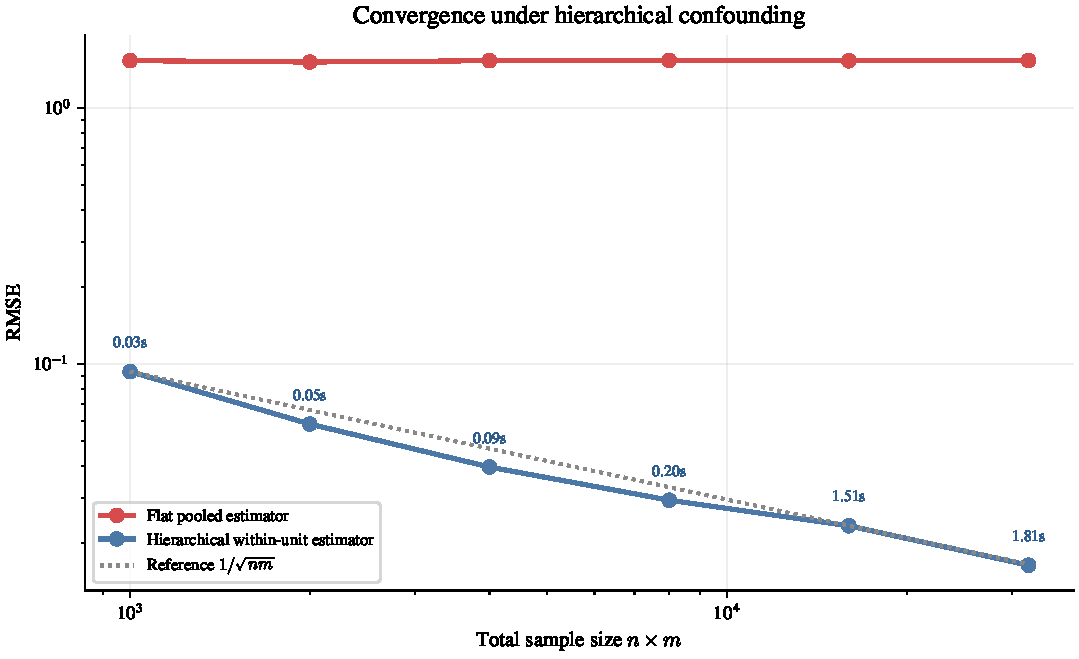
\includegraphics[width=0.78\textwidth]{synthetic_hcm_convergence_rmse.pdf}
\caption{Convergence diagnostic under hierarchical confounding. The flat pooled estimator does not approach the intervention target because the unit-level latent cause is ignored. The hierarchical within-unit estimator removes the unit effect and follows the expected $1/\sqrt{nm}$ decay as the total number of observations increases. Labels on the blue curve report the runtime for each simulated sample size.}
\label{fig:synthetic-convergence}
\end{figure}

\begin{table}[!htbp]
\centering
\small
\caption{Sequential versus parallel runtimes. Times are in seconds. The HCM rows are two-intervention evaluations from the STAR speed test; the OLS and IV rows are batched baseline workloads.}
\label{tab:parallel-runtime}
\begin{tabular}{lcccc}
\toprule
Workload & Sequential & 4 threads & 4 processes & Best speedup \\
\midrule
DirectLiNGAM HCM evaluation & 9.31 & 10.73 & 8.50 & $1.09\times$ \\
ExactBIC HCM evaluation & 3.11 & 3.63 & 1.90 & $1.64\times$ \\
OLS baseline batch & 12.32 & 6.71 & 0.46 & $26.77\times$ \\
IV baseline batch & 21.43 & 14.87 & 2.05 & $10.48\times$ \\
\bottomrule
\end{tabular}
\end{table}

Let $i=1,\ldots,n$ index units and $j=1,\ldots,m_i$ index sub-units.
For each sub-unit variable $L_{ij}$ with sub-unit parents $\pa_S(L)_{ij}$, the backend creates a unit-level $Q$-node
\begin{equation}
  Q_i^{L\g \pa_S(L)}
  =
  \pr\!\left(L_{ij}\g \pa_S(L)_{ij},\; \mathrm{unit}=i\right).
  \label{eq:qdef}
\end{equation}
Operationally, this equation is treated as a rule for constructing a new node name and its parents.
For example, an outcome mechanism $M\leftarrow(A,E,G,L)$ becomes the node $Q^{m\g a,e,g,l}$.
The backend stores this node as a variable of the collapsed graph, but its numerical value is only fitted later from the sub-unit table.
Thus equation~\eqref{eq:qdef} has two roles: graphically, it replaces a sub-unit mechanism by a unit-level variable; numerically, it declares which conditional density estimator will be needed.

The graph passed to pyAgrum is obtained through the HCM transformations.
Collapse replaces every sub-unit mechanism by its $Q$-node and lifts all edges to a flat directed acyclic graph over unit-level variables and $Q$-variables, denoted $G_{\col}$.
Augmentation then adds auxiliary $Q$-nodes for the target outcome, so that the outcome distribution is explicit in the collapsed graph; when required, marginalization projects out variables that are not part of the identification problem.
Only after these transformations is the graph copied into a pyAgrum DAG with the same nodes and directed arcs.
The treatment and outcome names are then passed to pyAgrum's do-calculus identification routine.
This means that pyAgrum never sees the original nested table: it sees the collapsed HCM graph and returns a symbolic expression for $\pr(Y\g\rmdo(X=x))$ in terms of observed variables of that graph.
Keeping this step separate from estimation is what allows the same identified expression to be evaluated later with Gaussian, mixture, categorical, non-parametric, or neural plug-in components.

The symbolic expression returned by pyAgrum is adapted into a typed AST and then written as the closed-form do-calculus formula used by the estimator.
Here AST means an abstract syntax tree: a nested object representation of the pyAgrum-identified formula after translation into HCM density factors, not only a string displayed in the paper.
Each node has a computational role.
A summation node stores the variables to marginalize; a product node stores the multiplicative factors; a conditional node stores one density key of the form $P(\mathrm{outcome}\g\mathrm{parents})$; and a leaf node is used for constants or fallback terms.
The do-calculus engine demo prints this adapted object directly.
For instance, one retained collapsed example identifies the formula shown below; the corresponding AST is the tree object printed by the backend:
\begin{center}
\setlength{\fboxsep}{7pt}
\begin{tabular}{@{}c@{\hspace{0.035\textwidth}}c@{}}
\textbf{Adapted AST} & \textbf{Identified formula} \\[4pt]
\fbox{%
\begin{minipage}[t]{0.43\textwidth}
\ttfamily\scriptsize
sum on Qz\_a,W for\par
\textbar{} *\par
\textbar{} \textbar{} *\par
\textbar{} \textbar{} \textbar{} P(W\textbar{}Qa)\par
\textbar{} \textbar{} \textbar{} P(Y\textbar{}Qa,Qz\_a,W)\par
\textbar{} \textbar{} sum on Qa for\par
\textbar{} \textbar{} \textbar{} *\par
\textbar{} \textbar{} \textbar{} \textbar{} P(Qz\_a\textbar{}Qa,W)\par
\textbar{} \textbar{} \textbar{} \textbar{} joint P(Qa)
\end{minipage}}%
&
\fbox{%
\begin{minipage}[t]{0.40\textwidth}
\vspace{0.35em}
\centering
\scriptsize
\[
\begin{aligned}
&\sum_{Q^{z\g a},W}
P(W\g Q^a)\,
P(Y\g Q^a,Q^{z\g a},W)\\
&\quad\times
\left[
\sum_{Q^a}
P(Q^{z\g a}\g Q^a,W)\,
P(Q^a)
\right].
\end{aligned}
\]
\vspace{0.35em}
\end{minipage}}%
\end{tabular}
\end{center}
This is the object used by the evaluator.
The first line is the outer marginalization node over $Q^{z\g a}$ and $W$.
The product node then has two children: a direct product of fitted conditionals, and an inner summation over $Q^a$.
Calling \texttt{collect\_conditionals()} on this tree returns the density keys $P(W\g Q^a)$, $P(Y\g Q^a,Q^{z\g a},W)$, $P(Q^{z\g a}\g Q^a,W)$, and $P(Q^a)$ that must be fitted or read from data.
Changing from $\rmdo(Q^a=1)$ to $\rmdo(Q^a=0)$ does not change the tree structure; it changes only the intervention value used when the same parsed tree is evaluated.
In larger formulas, this same mechanism may produce dozens of density keys and many repeated unit-level prediction problems.
Those tasks share the same formal estimand but do not need to be fitted as a single global regression, which is why the framework can scale to large nested datasets without changing the causal definition of the target.

\subsection{Evaluation and diagnostics}

The general target is
\begin{equation}
  \tau(q_1,q_0)
  =
  \E{Q^Y\g \rmdo(Q^a=q_1)}
  -
  \E{Q^Y\g \rmdo(Q^a=q_0)}.
  \label{eq:ate}
\end{equation}
In the implementation, equation~\eqref{eq:ate} is evaluated by copying the identified AST twice.
The first copy fixes the intervention node at $Q^a=q_1$, the second fixes it at $Q^a=q_0$, and the ATE is the difference between the two numerical evaluations.
For a backdoor-like confounder motif, this procedure reduces to the familiar unit-averaged plug-in estimator
\begin{equation}
  \widehat \tau(q_1,q_0)
  =
  \frac{1}{n}\sum_{i=1}^n
  \left[
  \widehat\mu_i(q_1)-\widehat\mu_i(q_0)
  \right],
  \qquad
  \widehat\mu_i(q)
  =
  \int y\, \widehat Q_i^{y\g a}(y\g q)\,\di y.
  \label{eq:plugin}
\end{equation}
Here, the outer average is an explicit loop over units.
The term $\widehat\mu_i(q)$ is produced by the estimator attached to the conditional $Q$-node $Q_i^{y\g a}$.
For parametric families the integral is analytic or quadrature-based; for simulation-based components the backend draws Monte Carlo samples and averages the predicted outcomes.
More complex graphs use the same evaluator, but the AST contains more density factors and more marginalization nodes.
Scalable estimation enters at exactly this point.
Each $\widehat\mu_i$ can be fitted from the sub-units of unit $i$, each conditional density factor can be estimated from its own parent set, and each branch of a sampled marginalization can be evaluated independently before the AST combines the results.
The computational structure therefore mirrors the statistical structure: many local estimators are assembled into one causal functional.

The canonical motifs used in the experiments serve as validation cases for this machinery.
They verify that pyAgrum identification, HCM formula adaptation, AST evaluation, and numerical evaluation agree on structures whose behaviour is known in advance.
In the confounder motif, for example, a latent unit variable affects both treatment and outcome mechanisms.
The collapsed graph contains $Q_i^a$ and $Q_i^{y\g a}$ as unit-level objects, and the intervention is evaluated by averaging the per-unit response:
\begin{equation}
  \E{Y\g \rmdo(Q^a=q_\star)}
  =
  \EE{i}{
    \int y\, Q_i^{y\g a}(y\g q_\star)\,\di y
  }.
  \label{eq:confounder-canonical}
\end{equation}
In the frontdoor/interference motif, an intermediate unit-level variable carries part of the causal pathway and the identified functional contains nested sums over the mediator distribution.
In the instrumental motif, the expression contains a reweighting term analogous to inverse probability weighting:
\begin{equation}
  \E{Y\g \rmdo(A\sim q_\star^a)}
  =
  \EE{Q^{a\g z},Q^z}{
    \frac{q_\star^a(a)}{Q^{a\g z}(a\g z)}\,Y
  },
  \label{eq:iv-canonical}
\end{equation}
provided the positivity conditions are met.
In the backend, the denominator $Q^{a\g z}(a\g z)$ is a fitted density node.
If this estimator is missing or has no support at the sampled value, the calculation becomes unstable.
This is why the implementation reports both the symbolic formula and factor-level diagnostics.

In practice, a symbolic formula may contain high-variance conditional density factors.
This can happen with multi-parent $Q$-variables, such as $Q^{m\g a,e,g,l}$, where the outcome distribution depends jointly on treatment, ethnicity, gender, and lunch status.
The implementation records such cases and, in the normalized-factor runs studied below, rescales unstable multiplicative factors before evaluation. Operationally this is a controlled truncation of the raw product scale: the graph structure is retained, but the unstable factor is normalized so that it cannot overwhelm the rest of the functional.
If the identified functional is $\mathfrak F$, the evaluated functional becomes a numerically stabilized object $\widetilde{\mathfrak F}$ with the same graph structure but normalized factor weights.
This is not a harmless implementation detail: normalizing $P(Z\g W)$ changes the weighting induced by that factor and therefore changes the numerical functional being evaluated.
We therefore report both the nominal identified formula and the factor normalization actually used in computation.

%% =============================================================================
\section{Experimental results}
\label{sec:experiments}
%% =============================================================================

\subsection{Canonical HCM motifs}

The experimental validation starts with three canonical motifs: confounding, confounding with interference/frontdoor structure, and an instrumental-variable design.
The data are generated from known HSCMs with $n=100$ units and $m=50$ sub-units; recovery of the causal contrast is shown in the convergence plot.
Appendix~\ref{app:software-notes} reports the parallel estimation structure for the same motifs.
Here $P$ denotes the number of CPU workers and $c$ denotes the average cost of one local density, response, or Monte Carlo evaluation task.
For a GPU implementation, the relevant parallelism is not a number of Python workers but a feasible tensor batch size, which depends on both $n$ and $m$.
We therefore treat GPU throughput as a hardware-specific Pareto frontier rather than as a fixed worker count.

The confounder experiment also varies the number of units.
With $m=50$ sub-units per unit, the estimate converges toward the true ATE as $n$ increases from 10 to 200, while pooled OLS remains biased because it mixes unit-level latent heterogeneity with the treatment effect.
This behaviour is important for interpretation: the HCM estimator is recovering the unit-level intervention encoded by the graph, rather than only fitting an association in the pooled student table.
It is also important computationally.
For these motifs, the expensive work consists of repeated unit-level response evaluations, factor evaluations, and Monte Carlo or quadrature branches.
These tasks are independent conditional on the identified AST, so the sequential work $T_1$ can ideally be reduced to $T_P\simeq T_1/P$ with $P$ CPU workers, up to scheduling overhead.
The same structure is highly GPU-parallelizable: units, sub-units, intervention values, and Monte Carlo samples are stacked into tensor batches and evaluated simultaneously when the density estimators are implemented in a tensor backend such as PyTorch or JAX\@.
The STAR timings reported below use CPU parallelism; Appendix~\ref{app:software-notes} gives the hardware-specific GPU Pareto benchmark used to document how the achievable batch frontier changes with $(n,m)$ on the available CUDA device.

\subsection{Do-calculus gallery}

The symbolic part of the pipeline is then checked on a gallery of identifiable binary HCM configurations.
Each configuration is identified automatically, converted to an AST, and evaluated numerically.
Because numerical ATE recovery is already shown by the convergence diagnostic, the gallery is shown graphically rather than repeated as a second numerical table.
Figure~\ref{fig:complete-instrument} displays the instrument motif in the main text because it shows the most distinctive HCM operation, namely marginalization after augmentation. The confounder and interference motifs are moved to Appendix~\ref{app:motif-figures} to keep the method section readable while still documenting the complete transformations.



\begin{figure}[!htbp]
\centering
\scriptsize
\begin{minipage}[t]{0.22\textwidth}
\centering
\textbf{(a) HCM}\par\medskip
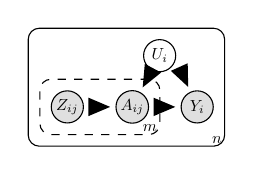
\begin{tikzpicture}[scale=0.58, transform shape]
\node[obs] (y) {$Y_{i}$};
\node[obs, left=0.7cm of y] (a) {$A_{ij}$};
\node[obs, left=0.7cm of a] (z) {$Z_{ij}$};
\node[latent, above=0.4cm of a, xshift=0.6cm] (u) {$U_i$};
\draw[hcmarrow] (a) -- (y);
\draw[hcmarrow] (u) to[bend left=12] (y);
\draw[hcmarrow] (u) -- (a);
\draw[hcmarrow] (z) -- (a);
\plate[dashed] {in} {(a)(z)} {$m$}
\plate {out} {(in)(u)(y)} {$n$}
\end{tikzpicture}
\end{minipage}\hspace{0.01\textwidth}
\begin{minipage}[t]{0.22\textwidth}
\centering
\textbf{(b) Collapsed}\par\medskip
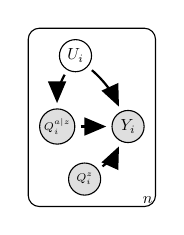
\begin{tikzpicture}[scale=0.58, transform shape]
\node[obs] (y) {$Y_{i}$};
\node[obs, left=0.8cm of y] (qaz) {$\scriptstyle Q^{a\mid z}_i$};
\node[obs, below=.4cm of qaz, xshift=0.6cm] (qz) {$\scriptstyle Q^{z}_i$};
\node[latent, above=0.8cm of qaz, xshift=0.4cm] (u) {$U_i$};
\draw[hcmarrow] (u) to[bend right=15] (qaz);
\draw[hcmarrow] (u) to[bend left=12] (y);
\draw[hcmarrow] (qaz) -- (y);
\draw[hcmarrow] (qz) to[bend right=15] (y);
\plate {out} {(qz)(qaz)(u)(y)} {$n$}
\end{tikzpicture}
\end{minipage}\hspace{0.01\textwidth}
\begin{minipage}[t]{0.22\textwidth}
\centering
\textbf{(c) Augmented}\par\medskip
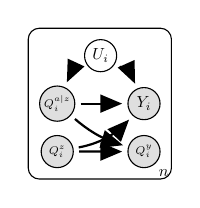
\begin{tikzpicture}[scale=0.58, transform shape]
\node[obs] (qaz) at (-0.95,0) {$\scriptstyle Q^{a\mid z}_i$};
\node[obs] (y) at (0.95,0) {$Y_i$};
\node[obs] (qz) at (-0.95,-1.05) {$\scriptstyle Q^{z}_i$};
\node[obs] (qy) at (0.95,-1.05) {$\scriptstyle Q^{y}_i$};
\node[latent] (u) at (0,1.05) {$U_i$};
\draw[hcmarrow] (u) to[bend right=18] (qaz);
\draw[hcmarrow] (u) to[bend left=18] (y);
\draw[hcmarrow] (qaz) -- (y);
\draw[hcmarrow] (qz) to[bend right=18] (y);
\draw[hcmarrow] (qaz) to[bend right=12] (qy);
\draw[hcmarrow] (qz) -- (qy);
\plate {out} {(qz)(qaz)(u)(y)(qy)} {$n$}
\end{tikzpicture}
\end{minipage}\hspace{0.01\textwidth}
\begin{minipage}[t]{0.22\textwidth}
\centering
\textbf{(d) Marginalized}\par\medskip
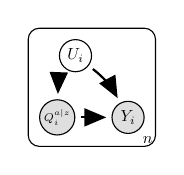
\begin{tikzpicture}[scale=0.58, transform shape]
\node[obs] (y) {$Y_{i}$};
\node[obs, left=0.8cm of y] (qaz) {$\scriptstyle Q^{a\mid z}_i$};
\node[latent, above=.6cm of qaz, xshift=0.4cm] (u) {$U_i$};
\draw[hcmarrow] (u) to[bend right=15] (qaz);
\draw[hcmarrow] (u) to[bend left=12] (y);
\draw[hcmarrow] (qaz) -- (y);
\plate {out} {(qaz)(u)(y)} {$n$}
\end{tikzpicture}
\end{minipage}
\caption{Complete graph transformations for the instrument motif. Marginalization removes $Q^z_i$, yielding the graph on which the do-calculus formula is evaluated.}
\label{fig:complete-instrument}
\end{figure}

\subsection{Representative benchmark scenarios}

Beyond the canonical motifs, additional synthetic checks are used as regression tests for the implementation rather than as a separate empirical contribution.
They cover binary HCMs, spatio-temporal HCMs, and grouped socioeconomic simulations with known targets; the numerical details are reported in Appendix~\ref{app:synthetic-benchmarks}.
The spatio-temporal checks are the most informative because the naive OLS estimate can be five to seven times larger than the true effect when a latent unit variable simultaneously affects baseline outcomes and treatment probability.
When the empirical estimand matches the theoretical one, the per-unit HCM estimator removes this source of bias.
When treatment interacts with context, however, the estimator reports the corresponding empirical target; this change in target is part of the interpretation rather than a numerical failure.
The convergence diagnostic in Figure~\ref{fig:synthetic-convergence} shows the same point visually: increasing $n\times m$ reduces RMSE for the hierarchical estimator, while the flat pooled estimator remains biased because the unit-level latent cause is still unmodelled.
The same benchmarks also demonstrate why the AST representation matters computationally: unit-level fits, factor evaluation, and Monte Carlo branches are independent tasks. Table~\ref{tab:parallel-runtime} compares sequential and parallel runs; on the STAR ExactBIC speed test, process-based parallelism reduced the two-intervention evaluation from $3.11$ seconds to $1.90$ seconds, a $1.64\times$ speedup. The current reported runs use CPU parallelism; the same decomposition is compatible with GPU-accelerated density estimators because batches of units and Monte Carlo samples can be evaluated independently.

%% =============================================================================
\section{Real data analysis: Project STAR}
\label{sec:star}
%% =============================================================================

\subsection{Data and hierarchical representation}

\begin{center}
\captionof{table}{STAR HCM estimates and normalized-factor diagnostic. The Mathematics row is the main outcome analysis; the Reading row is a separate diagnostic run used to inspect the normalized $P(Q^{y\g a,g}\g S)$ factor.}
\label{tab:hcmstar}
\begin{tabular}{llccc}
\toprule
Run & Target & $E[\rmdo(1)]$ & $E[\rmdo(0)]$ & ATE \\
\midrule
ExactBIC & Mathematics ($M$) & 2402.75 & 2365.95 & 36.80 \\
ExactBIC, normalized factors & Reading ($Y$) diagnostic & 1788.10 & 1766.47 & 21.63 \\
\bottomrule
\end{tabular}
\end{center}

Project STAR randomized kindergarten students within schools to small classes, regular classes, or regular classes with an aide.
The full STAR-and-Beyond public-use dataset is documented by \citet{Achilles2008} and distributed through Harvard Dataverse at \href{https://doi.org/10.7910/DVN/SIWH9F}{this link}; it contains the raw student- and school-level records from the longitudinal Tennessee experiment, including demographics, class assignments, school identifiers, teacher information, and achievement outcomes.
After removing missing values, the kindergarten cohort contains 5,745 student records across 322 classes and 79 schools; for the class-as-unit HCM analysis and diagnostics, the scripts then use a balanced sample of 10 students per class, yielding 3,220 student records across 322 classes.
The main outcome in this paper is Mathematics ($M$), measured by the STAR score \texttt{gktmathss}, but Reading ($Y$), measured by \texttt{gktreadss}, is retained because it enters some discovered graph structures and appears in the identified HCM formulas.
Classes are treated as units and students as sub-units.
The treatment is the student-level small-class assignment, written $A_{ij}=\mathbf 1\{\mathrm{small\ class}\}$, with student covariates given by Gender ($G_{ij}$), Ethnicity ($E_{ij}$), and Free-lunch status ($L_{ij}$).
School urbanicity ($S_i$) is treated as an observed class-level covariate, while $U_i$ collects all unobserved unit-level causes, including but not limited to class heterogeneity, latent school context, teacher effects, and other shared classroom factors.
The intervention is therefore not a row-level replacement of $A_{ij}$, but a class-level intervention $\rmdo(Q^a=q_\star^a)$ that fixes the small-class assignment distribution within the class.
In plain terms, the $Q$-quantities used below are class summaries of student-level variables: $Q^a$ is the small-class assignment probability or proportion in a class, $Q^g$ is the gender composition, and Gaussian score mechanisms such as $Q^m$ or $Q^y$ are represented by fitted class-specific means and variances.

\begin{center}
\centering
\scriptsize
\begin{tabular}{ccccccccc}
\toprule
\texttt{stdntid} & \texttt{gktchid} & $S_i$ & $A_{ij}$ & $G_{ij}$ & $E_{ij}$ & $L_{ij}$ & $Y_{ij}$ & $M_{ij}$ \\
\midrule
11311 & 11203801 & 4 & 1 & 1 & 1 & 1 & 413 & 454 \\
\bottomrule
\end{tabular}
\captionof{table}{Example row from the balanced STAR HCM sample. The row is shown after recoding the raw kindergarten variables into the symbols used by the HCM analysis.}
\label{tab:star-example-row}
\end{center}

\begin{figure}[!htbp]
\centering
\begin{minipage}[t]{0.34\textwidth}
\centering
\vspace{0pt}
\scriptsize
\setlength{\tabcolsep}{2pt}
\begin{tabular}{lll}
\toprule
Symbol & Level & Definition \\
\midrule
$A$ & student & Small-class assignment, \texttt{stark} \\
$M$ & student & Mathematics score, \texttt{gktmathss} \\
$Y$ & student & Reading score, \texttt{gktreadss} \\
$G$ & student & Gender indicator, \texttt{gender} \\
$E$ & student & Ethnicity indicator, \texttt{ethnicity} \\
$L$ & student & Free-lunch status, \texttt{lunchk} \\
$S$ & class & School urbanicity, \texttt{schoolk} \\
$U$ & latent & Unobserved class heterogeneity \\
\bottomrule
\end{tabular}
\captionof{table}{STAR variables used in the HCM analysis.}
\label{tab:variables}
\vspace{0.8em}
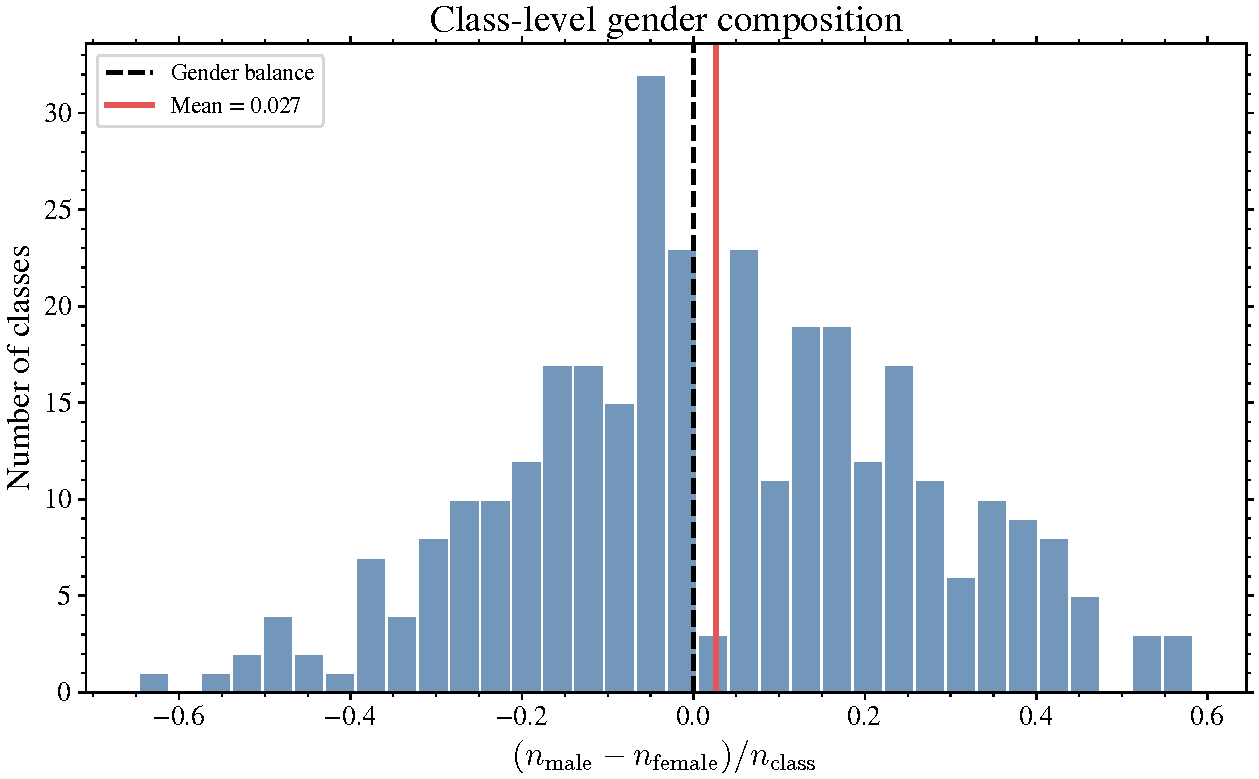
\includegraphics[width=\linewidth]{class_gender_heterogeneity_distribution.pdf}
\end{minipage}\hfill
\begin{minipage}[t]{0.62\textwidth}
\centering
\vspace{0pt}
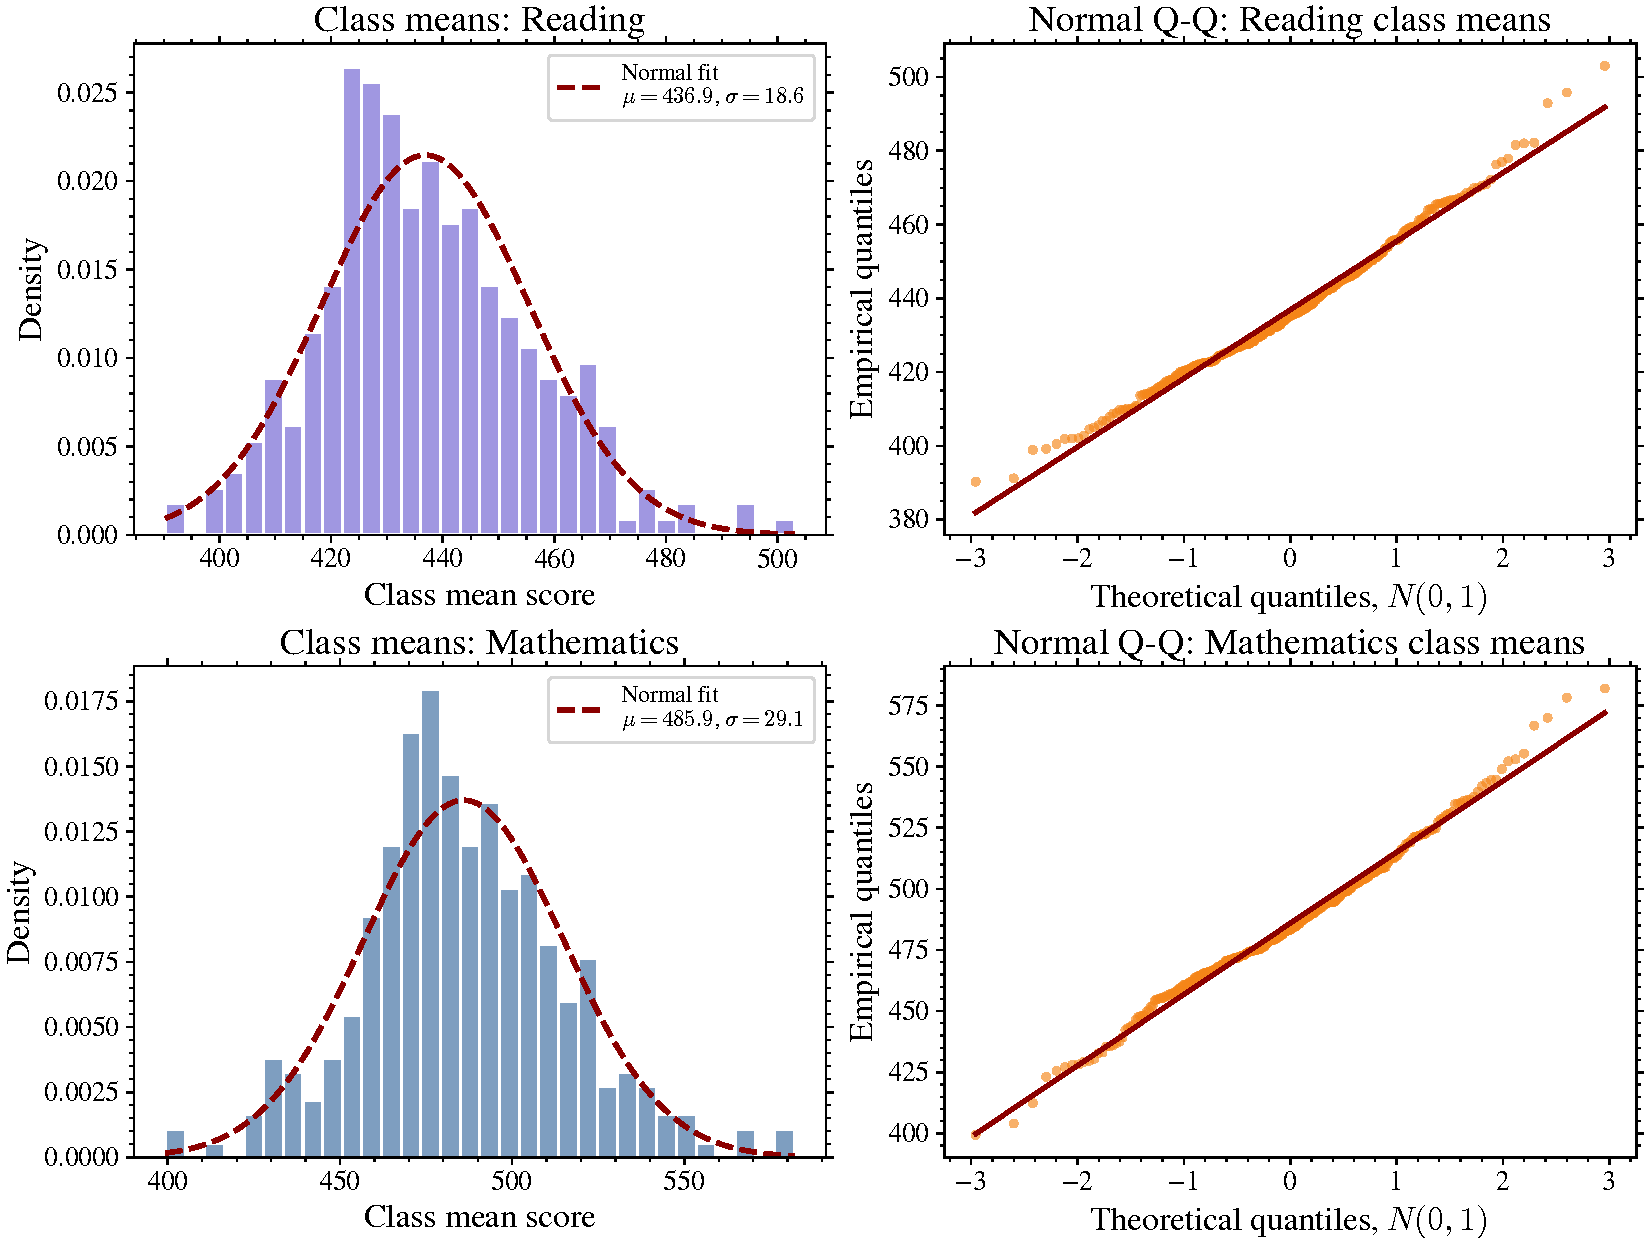
\includegraphics[width=\linewidth]{class_level_means_Y_M_gaussian_lognorm.pdf}
\end{minipage}
\caption{Class-level STAR diagnostics. Left: gender heterogeneity across classes, showing why an additive individual gender coefficient does not represent the full distribution of class composition. Right: reading and mathematics class-level score means, with histograms and Q-Q plots used to assess Gaussian plug-in choices for $Q$-variables.}
\label{fig:gender-heterogeneity}
\label{fig:class-level-means}
\end{figure}

\begin{figure}[!htbp]
\centering
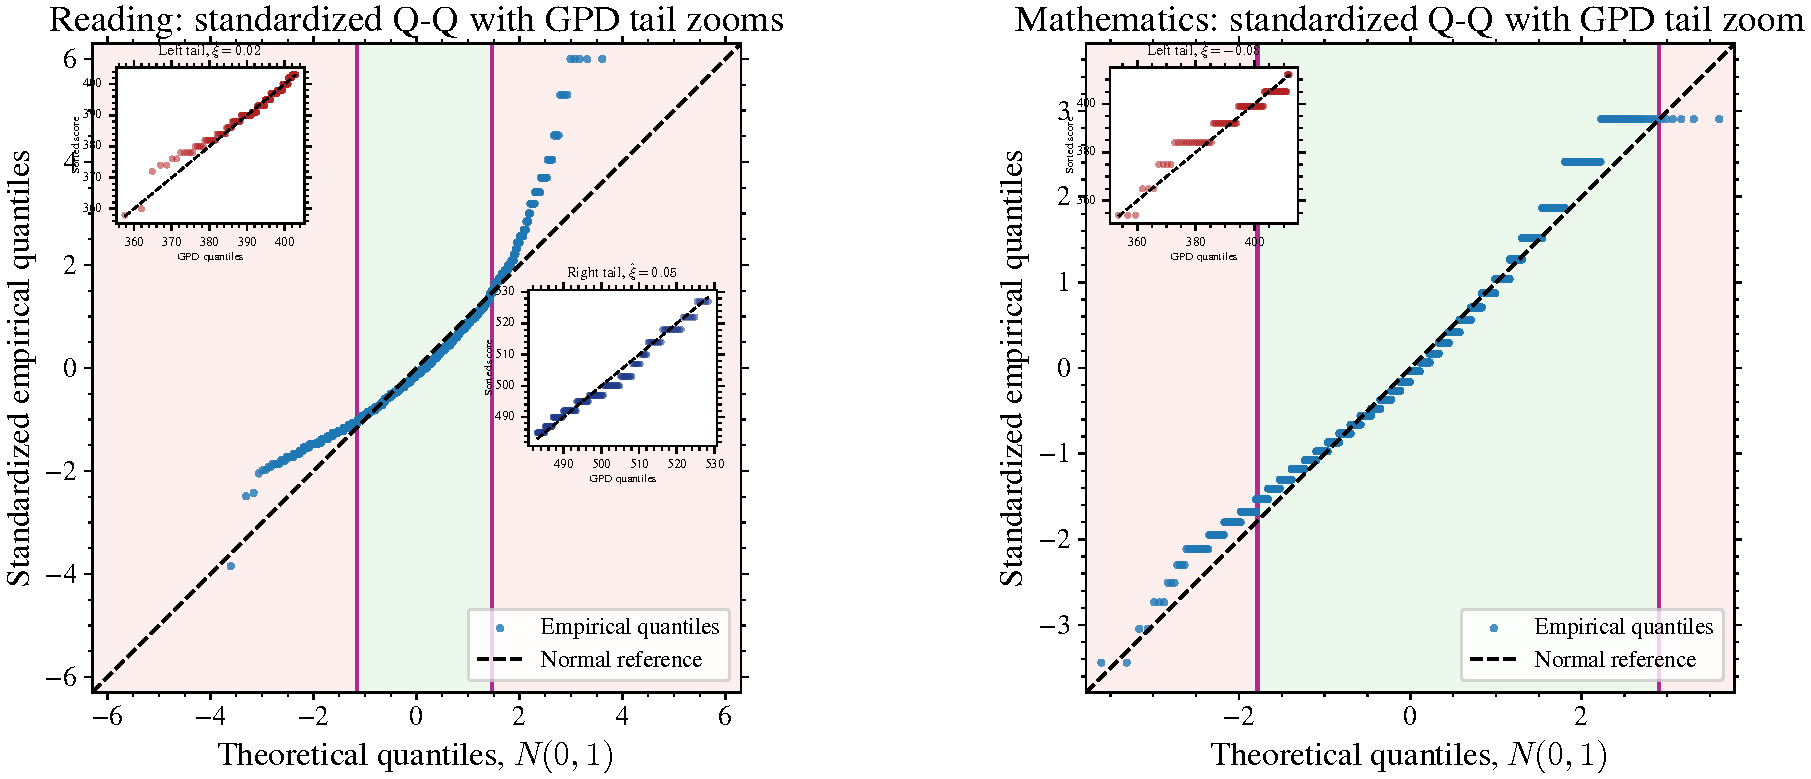
\includegraphics[width=0.86\textwidth]{global_Y_M_heavy_tail_qq.pdf}
\caption{Heavy-tail Q-Q diagnostics for Reading ($Y$) and Mathematics ($M$). In each main panel, standardized empirical score quantiles are compared with theoretical Gaussian quantiles; systematic bending away from the diagonal indicates that a single global Gaussian approximation is too light-tailed in the extremes. The inset subplots zoom separately on the lower and upper tails and compare the empirical tail behaviour with a generalized Pareto distribution (GPD) diagnostic, making the extreme-score departures visible rather than hidden by the central mass.}
\label{fig:score-qq-diagnostics}
\end{figure}

\subsection{Baseline regressions}

As baselines, we reproduce the standard student-level regression contrasts used in the STAR literature and compare them with a non-causal hierarchical reading of the data.
The OLS replication starts from the pooled contrast
\begin{align}
  M_i
  &=
  \alpha
  + \beta_1\,\mathrm{small}_i
  + \beta_2\,\mathrm{reg\_aide}_i
  + \varepsilon_i ,
  \label{eq:ols-pooled}
\end{align}
then adds school fixed effects,
\begin{align}
  M_i
  &=
  \alpha
  + \beta_1\,\mathrm{small}_i
  + \beta_2\,\mathrm{reg\_aide}_i
  + \delta_{\mathrm{school}(i)}
  + \varepsilon_i ,
  \label{eq:ols-school}
\end{align}
and finally includes student and teacher controls. The richest specification is
\begin{align}
  M_i
  &=
  \alpha
  + \beta_1\,\mathrm{small}_i
  + \beta_2\,\mathrm{reg\_aide}_i
  + \gamma^\top X_i
  + \delta_{\mathrm{school}(i)}
  + \varepsilon_i ,
  \label{eq:ols}
\end{align}
where $X_i$ includes race, gender, free-lunch status, teacher race, teacher experience, and teacher education.
The coefficient $\beta_1$ is therefore a student-level small-class contrast, conditional on the chosen controls.

\begin{center}
\captionof{table}{OLS estimates of the small-class effect on kindergarten mathematics.}
\label{tab:ols}
\begin{tabular}{lcccc}
\toprule
Model & $\hat\beta_{\mathrm{small}}$ & SE & $p$-value & $R^2$ \\
\midrule
No controls & 8.096 & 1.597 & $4.0\times 10^{-7}$ & 0.006 \\
School fixed effects & 9.499 & 1.463 & $8.5\times 10^{-11}$ & 0.219 \\
Student controls & 9.380 & 1.415 & $3.4\times 10^{-11}$ & 0.268 \\
Full OLS replication & 9.432 & 1.419 & $3.0\times 10^{-11}$ & 0.269 \\
\bottomrule
\end{tabular}
\end{center}

The instrumental-variable replication uses assignment indicators as instruments for actual class size. In first stage,
\begin{align}
  \mathrm{classsize}_i
  &=
  \pi_0
  + \pi_1\,\mathrm{small}_i
  + \pi_2\,\mathrm{reg\_aide}_i
  + \Pi^\top X_i
  + \delta_{\mathrm{school}(i)}
  + \nu_i ,
  \label{eq:first-stage}
\end{align}
and the second stage estimates
\begin{align}
  M_i
  &=
  \alpha
  + \theta\,\widehat{\mathrm{classsize}}_i
  + \gamma^\top X_i
  + \delta_{\mathrm{school}(i)}
  + \varepsilon_i,
  \label{eq:second-stage}
\end{align}
This gives a second-stage coefficient of $-1.219$ mathematics points per additional student (SE $0.163$).
The corresponding non-causal hierarchical regression baseline can be written as a random-intercept or Bayesian OLS model,
\begin{align}
  M_{ij}
  &=
  \alpha
  + \beta_1\,\mathrm{small}_{ij}
  + \beta_2\,\mathrm{reg\_aide}_{ij}
  + \gamma^\top X_{ij}
  + b_{\mathrm{class}(i)}
  + \varepsilon_{ij},
  \qquad
  b_c \sim \mathcal{N}(0,\sigma_b^2).
  \label{eq:hierarchical-baseline}
\end{align}
This model is valuable because it acknowledges between-class heterogeneity, but it treats that heterogeneity as a residual random effect rather than as a distributional causal mechanism.
In other words, the model can say that some classes have higher or lower baseline mathematics scores, and OLS can adjust for observed individual covariates such as gender or free lunch, but neither model represents the class as an object whose internal composition changes the intervention itself.
The heterogeneity is absorbed into fixed effects, controls, or random intercepts; it is not decomposed into class-level $Q$-mechanisms such as the treatment distribution $Q^a$, gender composition $Q^g$, or response factors depending jointly on treatment and composition.
This is precisely where a causal HCM analysis becomes necessary.
For STAR, the scientific question is not only whether an individual assigned to a small class has a different expected score, but how a class-level intervention on the distribution of small-class assignment propagates through heterogeneous classroom mechanisms.
OLS, IV, and hierarchical Bayesian/OLS baselines therefore include gender and class variation descriptively, but they do not treat class composition or treatment-by-gender mechanisms as intervention-level distributions.
This distinction motivates the HCM diagnostics below.

\subsection{HCM under discovered graphs}

\begin{figure}[!htbp]
\centering
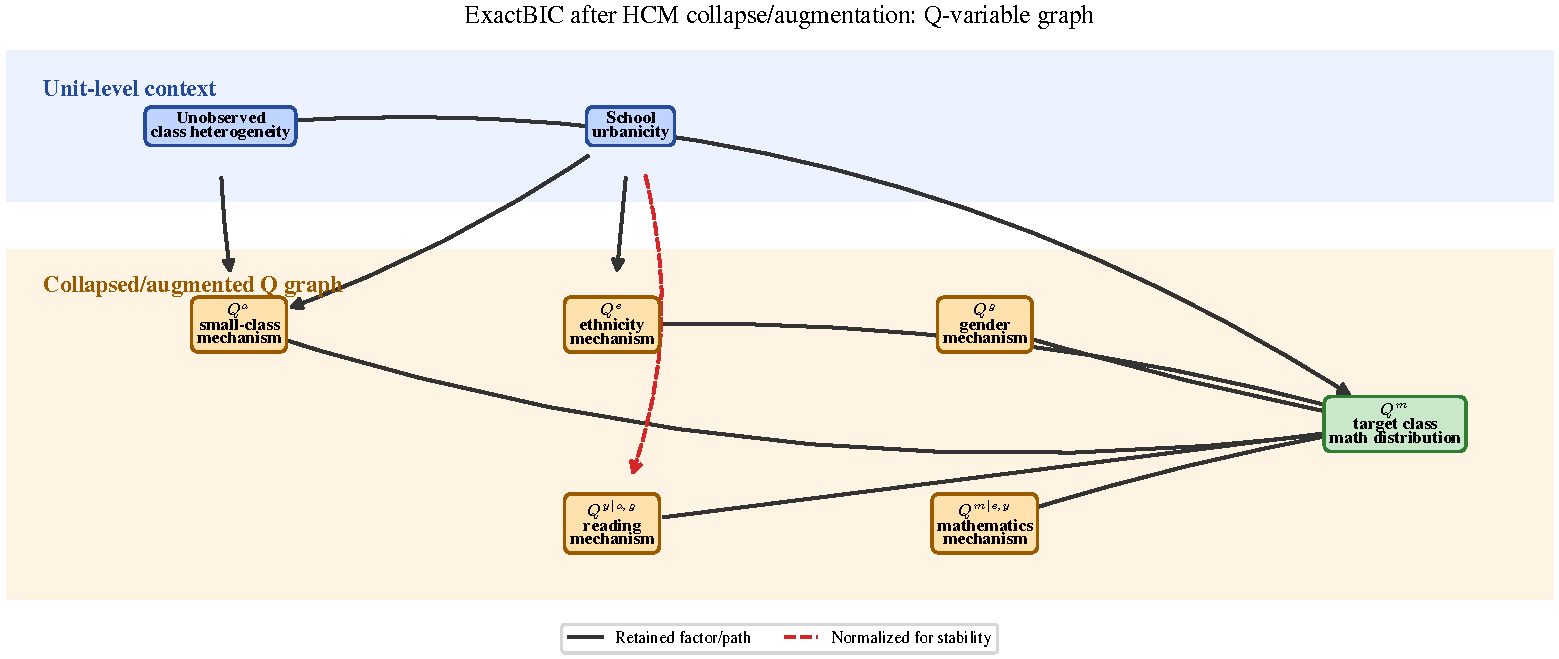
\includegraphics[width=0.96\textwidth]{ExactBIC_transformed_q_graph.pdf}
\caption{ExactBIC graph after HCM collapse and augmentation for the mathematics target. Student-level variables are represented by class-level mechanisms $Q$; the green node is the target class-level Mathematics distribution $Q^m$ evaluated under $\rmdo(Q^a=q_\star^a)$. The dashed red arrow indicates the $P(Q^{y\g a,g}\g S)$ factor normalized in the stabilized ExactBIC run.}
\label{fig:exactbic-q-graph}
\end{figure}

The STAR HCM analysis starts from graph structures learned on the flat discovery variables
\[
  (\texttt{readk},\texttt{mathk},\texttt{stark},\texttt{gender},\texttt{ethnicity},\texttt{lunchk},\texttt{schoolk}).
\]
For the ExactBIC run, we used one score-based DAG stored in the discovery output, with the school-urbanicity/ethnicity relation oriented as Urbanicity ($S$) $\to$ Ethnicity ($E$) for substantive interpretability. This is one plausible graph, not a claim that the discovery step has recovered a unique causal structure.
The directed edges were translated through the fixed map
\[
\texttt{stark}\mapsto \text{Small-class assignment }(A),\quad
\texttt{readk}\mapsto \text{Reading }(Y),\quad
\texttt{mathk}\mapsto \text{Mathematics }(M),
\]
\[
\texttt{gender}\mapsto \text{Gender }(G),\quad
\texttt{ethnicity}\mapsto \text{Ethnicity }(E),\quad
\texttt{lunchk}\mapsto \text{Free lunch }(L),\quad
\texttt{schoolk}\mapsto \text{Urbanicity }(S).
\]
Thus the ExactBIC graph used here contains the translated dependencies
Reading ($Y$) $\to$ Mathematics ($M$), Mathematics ($M$) $\to$ Free lunch ($L$), Small-class assignment ($A$) $\to$ Reading ($Y$), Gender ($G$) $\to$ Reading ($Y$), Ethnicity ($E$) $\to$ Mathematics ($M$), Ethnicity ($E$) $\to$ Free lunch ($L$), Urbanicity ($S$) $\to$ Ethnicity ($E$), Urbanicity ($S$) $\to$ Reading ($Y$), Urbanicity ($S$) $\to$ Small-class assignment ($A$), and Urbanicity ($S$) $\to$ Free lunch ($L$).
Before identification, the HCM construction also adds the latent class-level confounding edges Unobserved class heterogeneity ($U$) $\to$ Small-class assignment ($A$) and Unobserved class heterogeneity ($U$) $\to$ Mathematics ($M$), because the target outcome in this paper is Mathematics ($M$).
The resulting hierarchical graph is then collapsed and augmented for $Q^m$ (the class-level Mathematics mechanism), giving the $Q$-variable graph in Figure~\ref{fig:exactbic-q-graph}; this transformed graph is passed to pyAgrum and evaluated with the plug-in families used in the run: Bernoulli models for Small-class assignment ($A$), Gender ($G$), Ethnicity ($E$), and Free lunch ($L$), a categorical model for Urbanicity ($S$), and two-component Gaussian mixtures for Reading ($Y$) and Mathematics ($M$).
After this translation, the class-as-unit HCM v2 model gives the estimates reported in Table~\ref{tab:hcmstar}, together with the separate normalized-factor diagnostic for the Reading mechanism.

These values should not be read as direct replacements for the student-level OLS coefficient, but the comparison is still essential.
OLS gives a student-level contrast for a binary treatment indicator, conditional on observed covariates and school fixed effects; IV gives a class-size contrast using assignment as an instrument.
The HCM estimand is instead a class-level intervention on $Q^a$, with additional dependence through class-specific distributions.
The fact that the ExactBIC HCM contrast remains much larger than the OLS coefficient is a warning sign: once the hierarchy is ignored, the target no longer contains the class-composition mechanisms that drive the HCM functional.
The HCM magnitude therefore describes the behaviour of the translated hierarchical estimand, while the separate normalized-factor diagnostic below shows that the numerical result is sensitive to the scaling of multiplicative factors retained in the identified formula.

\begin{figure}[!htbp]
\centering
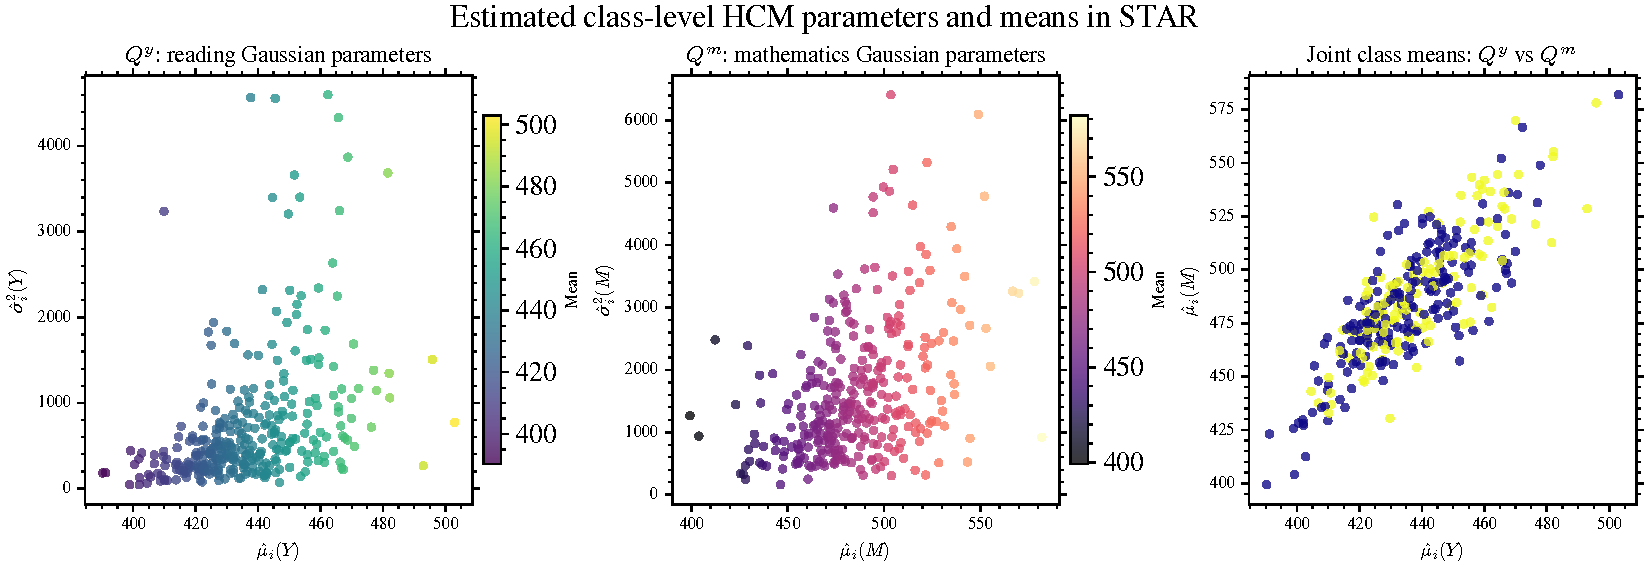
\includegraphics[width=0.88\textwidth]{enriched_q_parameters_means_star.pdf}
\caption{Estimated class-level HCM response parameters and means in STAR\@. Reading ($Q^y$) and Mathematics ($Q^m$) are represented by Gaussian summaries $(\hat\mu_i,\hat\sigma_i^2)$, and the right panel reports the joint class means used to inspect the relationship between the two score mechanisms.}
\label{fig:q-parameters-means}
\end{figure}

Figure~\ref{fig:q-parameters-means} shows that the response mechanisms are not constant across classes.
For both Reading and Mathematics, classes with larger fitted means also tend to have larger fitted variances, so the Gaussian $Q$-summaries capture both level differences and heteroskedasticity across classrooms.
This matters for the HCM plug-in estimator because an intervention on the class-level treatment distribution is evaluated through these class-specific response mechanisms, not through a single pooled outcome regression.
The right panel shows a strong positive association between class-level Reading and Mathematics means, indicating that the two achievement mechanisms share substantial classroom-level structure.
Consequently, the mathematics effect should not be interpreted as an isolated student-level coefficient: it is evaluated in a distribution of classrooms whose baseline achievement and score variability differ markedly.

\subsection{Identified formulas for STAR}

The ExactBIC-derived graph gives the following functional after the translated graph has been collapsed and augmented for the mathematics outcome:
\begin{align}
\tau_{\mathrm{BIC}}(q^a_\star)
&=
\sum_{q^e,q^g,q^{m\g e,y},q^{y\g a,g},s}
\pr(q^e\g s)
\pr(q^{y\g a,g}\g s)
\pr(q^{m\g e,y})
\nonumber\\
&\quad\times
\E{Q^m \g Q^a=q^a_\star,Q^e,Q^g,Q^{m\g e,y},Q^{y\g a,g}}
\pr(q^g)\pr(s).
\label{eq:bicstar}
\end{align}
In this expression, $\pr(q^{m\g e,y})$ is the class-level Mathematics ($M$) distribution induced by the discovered Reading ($Y$) $\to$ Mathematics ($M$) and Ethnicity ($E$) $\to$ Mathematics ($M$) parents, $\pr(q^e\g s)$ encodes the substantively oriented Urbanicity ($S$) $\to$ Ethnicity ($E$) relation, and $\pr(q^{y\g a,g}\g s)$ comes from the Reading ($Y$) mechanism with Small-class assignment ($A$), Gender ($G$), and Urbanicity ($S$) in the translated graph.
The expectation term is evaluated twice, at $Q^a=1$ and $Q^a=0$, and the remaining $Q$-variables are marginalized by the product of fitted density factors.
The formula therefore makes clear why multi-parent $Q$-estimation matters: the identified effect is a product of conditional densities and outcome-response factors, not a single regression coefficient.

\subsection{Effective graphs and factor normalization}

The normalized-factor diagnostic in Table~\ref{tab:hcmstar} makes explicit the difference between a nominal identified functional and the stabilized functional actually evaluated by the numerical code.
For ExactBIC, the diagnostic run concerns the Reading ($Y$) mechanism and the normalized term was $P(Q^{y\g a,g}\g S)$, which is the distribution of the class-level Reading mechanism conditional on Small-class assignment ($A$) and Gender ($G$), further conditioned by Urbanicity ($S$).
Normalizing such a factor does not remove variables from the nominal causal graph, but it rescales the corresponding weighting in the product that is numerically evaluated.
The effective graph in Figure~\ref{fig:exactbic-effective-graph} visualizes this distinction: dashed red arrows are dependencies present in the nominal graph whose factor contribution is normalized in the stabilized functional.

The ExactBIC gender factor analysis clarifies what this means numerically.
In Table~\ref{tab:hcmstar}, the normalized factor $P(Q^{y\g a,g}\g S)$ is stabilized before the two intervention evaluations, so its raw scale does not dominate the product. The corresponding factor-level traces vary on roughly $10^3$ scales in the raw product, which is precisely the numerical symptom that motivates the normalized analysis.
It nevertheless marks an important part of the estimand: the graph says that the class-level Reading ($Y$) response should depend on Small-class assignment ($A$), Gender ($G$) composition, and Urbanicity ($S$).
When the same run is analysed in unit context, the only non-zero factor change comes from the fitted response term $P(Q^y\g Q^a,Q^g,Q^{y\g a,g})$, namely Reading ($Y$) conditional on Small-class assignment ($A$), Gender ($G$), and the class-level Reading mechanism $Q^{y\g a,g}$, whose mean changes from $434.83$ under $\rmdo(Q^a=0)$ to $440.15$ under $\rmdo(Q^a=1)$.
The resulting delta, $5.32$, explains why the gender mechanism matters even when the conditional factor is normalized for stability.

\subsection{Diagnostics and interpretation}

The STAR analysis also illustrates why diagnostics are essential.
The experiments expose a central operational issue: an identified formula may contain multi-parent $Q$-variables whose density factors are numerically unstable.
In the normalized-factor runs, the evaluator rescales these multiplicative factors to keep the product stable and comparable across interventions.
In the ExactBIC STAR run, the normalized factor was the gender-dependent term $P(Q^{y\g a,g}\g S)$.
The diagnostic is scientifically useful only when it is read at the factor level: factor levels show which terms dominate the product numerically, while unit-context factor changes show which term changes between the two interventions.
The score distributions have heavy, non-Gaussian tails, so Figure~\ref{fig:score-qq-diagnostics} reports tail diagnostics rather than relying only on a global Gaussian approximation; the corresponding histogram diagnostic is given in Appendix~\ref{app:tail-diagnostics}.
In Figure~\ref{fig:score-qq-diagnostics}, the main Q-Q panels diagnose the whole standardized score distribution, while the inset subplots focus on the lower and upper extremes through GPD tail zooms.
This split is important: a Gaussian plug-in can look acceptable near the centre of Reading ($Y$) and Mathematics ($M$), but still underrepresent rare low or high classroom scores that affect fitted $Q$-response factors and product-form HCM evaluations.
The gender-composition diagnostic in Figure~\ref{fig:gender-heterogeneity} shows that class composition varies substantially across classes; an OLS coefficient on \texttt{female} adjusts for an average individual difference, but it does not represent the distribution of class composition.
HCM explicitly represents such within-class distributions through the estimated probability $Q$-quantities in Figure~\ref{fig:q-probabilities} and the response parameters and means in Figure~\ref{fig:q-parameters-means}.
The ExactBIC factor analysis above shows how gender composition enters the intervention path through $Q^{y\g a,g}$.
The current implementation remains two-level and treats schools only through unit-level covariates rather than as a full student--class--school hierarchy.
This is the main substantive lesson of the STAR analysis.
Earlier non-causal hierarchical or graphical summaries could describe that classes differ, but they did not make class heterogeneity part of an identified intervention functional.
By combining class-level $Q$-heterogeneity with factor analysis of the identified formula, the HCM pipeline shows that part of the small-class effect can be hidden when class composition and multi-parent distributional factors are treated only as background variation.
In that sense, the previous hierarchical graph analysis tended to smooth or understate the intervention contrast, whereas the causal HCM analysis gives a new interpretation of STAR: the effect of class size is not only an average student-level coefficient, but a distributional class-level effect whose magnitude depends on which class mechanisms are included, estimated, or normalized in the plug-in functional.

\begin{figure}[!htbp]
\centering
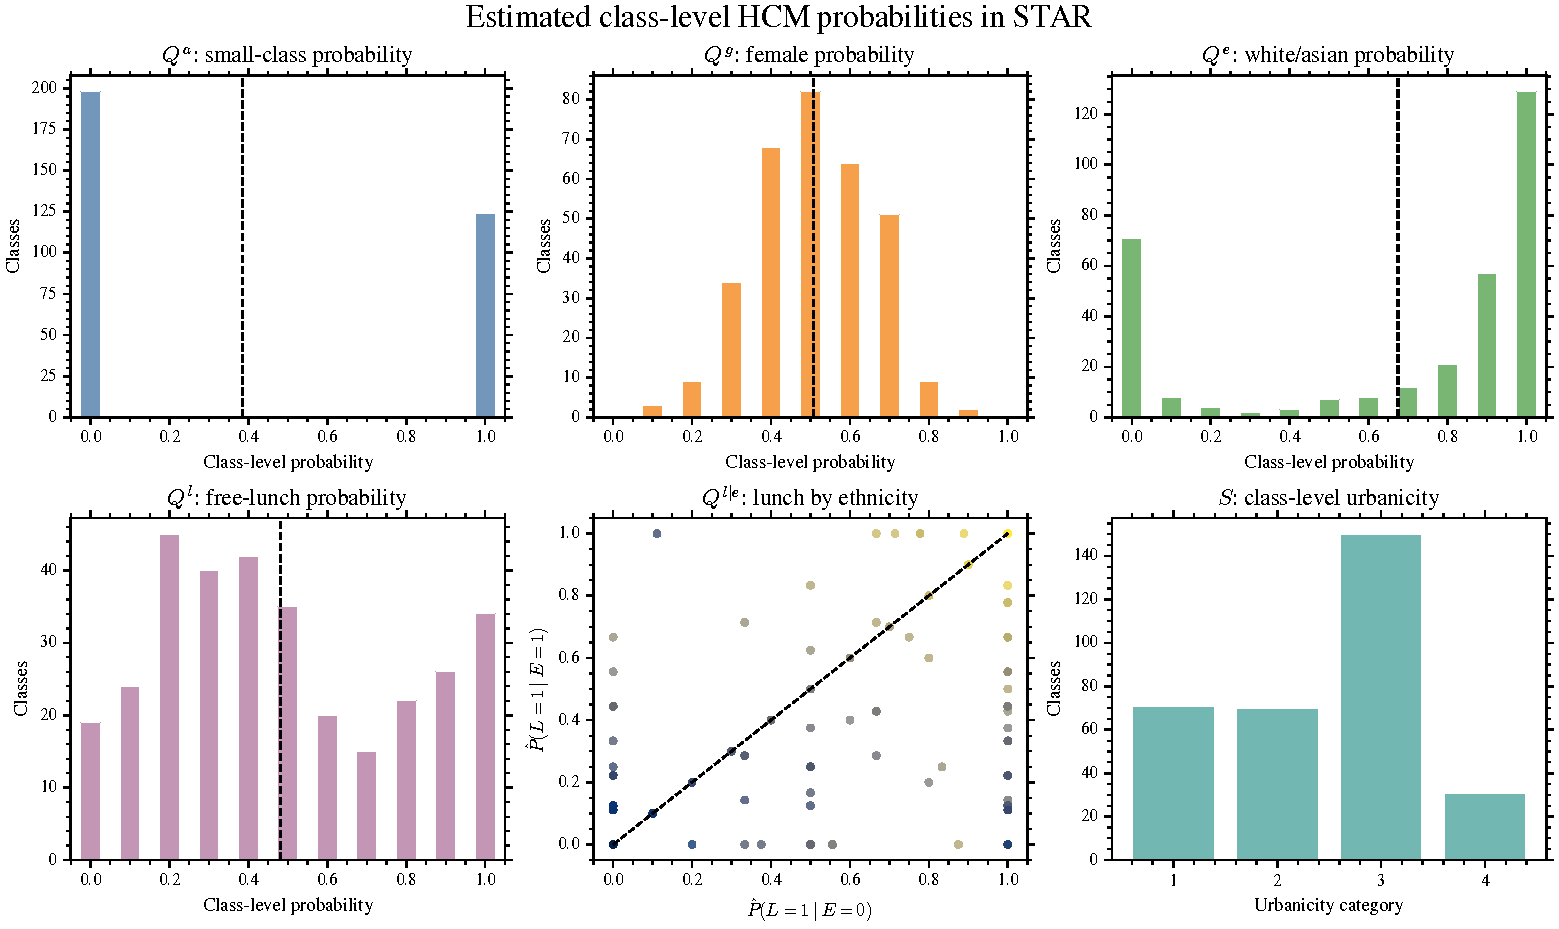
\includegraphics[width=0.88\textwidth]{enriched_q_probabilities_star.pdf}
\caption{Estimated class-level HCM probability quantities used in the STAR plug-in analysis. Binary sub-unit variables are represented by class-level Bernoulli probabilities for Small-class assignment ($Q^a$), Gender ($Q^g$), Ethnicity ($Q^e$), and Free lunch ($Q^l$); $Q^{l\g e}$ summarizes the Free-lunch mechanism conditional on Ethnicity; and $S$ is the observed class-level Urbanicity variable.}
\label{fig:q-probabilities}
\end{figure}

The substantive conclusion is therefore conservative.
HCM does not simply ``improve'' OLS by producing a larger number; it changes the estimand from a student-level coefficient to a distributional class-level intervention.
In STAR this change is scientifically meaningful, but it also makes graph choice, positivity, and plug-in completeness part of the reported result rather than secondary implementation details.

%% =============================================================================
\section{Conclusion}
\label{sec:conclusion}
%% =============================================================================

We developed a scalable automatic identification and estimation implementation for hierarchical causal inference.
The pipeline starts from a hierarchical graph, applies the HCM transformations needed for identification, obtains a symbolic do-calculus estimand from pyAgrum, adapts it into closed-form HCM formulas, and evaluates the associated AST using plug-in density estimators.
This turns HCM from a formal identification framework into an operational workflow for nested data.
The key computational point is that the AST does not leave the formula as an opaque expression: it decomposes the estimand into many local conditional densities, response models, and marginalization branches that can be estimated independently and then recombined into a single causal functional.
The implementation is available at \href{https://github.com/AI-vidence/hierarchicalcausalmodels}{\texttt{AI-vidence/hierarchicalcausalmodels}}, so the graph transformations, identification calls, estimators, diagnostics, and STAR replication artefacts can be inspected and reused.

The experiments validate the pipeline on known structures and reveal the practical regimes in which estimation is stable.
The STAR application demonstrates the methodological payoff: when the intervention is assigned at the class level and outcomes are measured at the student level, the natural estimand is hierarchical.
OLS, IV, and non-causal hierarchical summaries remain essential benchmarks, but they do not encode interventions on within-class treatment distributions or class-composition mechanisms.
The same framework also clarifies why large hierarchical applications are computationally feasible: adding units, factors, or sampled branches increases the number of local estimation tasks, but it does not require redefining the estimand or replacing it by a flat pooled regression.

The remaining limitations point directly to the next statistical developments.
The present implementation is two-level, whereas STAR is naturally a student--class--school system; extending scalable HCM estimation to deeper hierarchies is therefore necessary for a fully faithful education application.
Multi-parent $Q$-density estimation is the main statistical bottleneck, because missing or weakly estimated factors change the effective estimand rather than merely adding numerical noise.
Uncertainty quantification for normalized or otherwise stabilized functionals also remains open.
Future work should therefore develop robust multi-parent estimators, extend the implementation to deeper hierarchies, preserve the parallel structure of the AST evaluator, and connect the numerical backend to symbolic DSLs such as \texttt{y0} so that formula manipulation and estimation can share a common representation. For discovery-driven applications, the next step is to evaluate families of plausible DAGs rather than a single graph, using cluster-DAG ideas to group graphs that agree on coherent blocks of variables and to report how the HCM estimand changes across those graph clusters.

%% =============================================================================
\section*{Author contributions}
All authors contributed to methodology, software, experiments, and writing.

\section*{Data availability}
The full Project STAR public-use data are available as the STAR-and-Beyond dataset documented by \citet{Achilles2008} and hosted by Harvard Dataverse at \href{https://doi.org/10.7910/DVN/SIWH9F}{this link}. Code and generated artefacts are maintained at \href{https://github.com/AI-vidence/hierarchicalcausalmodels}{this link}.

\begin{thebibliography}{99}

\bibitem[Achilles et al.(2008)]{Achilles2008}
C. Achilles, H. P. Bain, F. Bellott, J. Boyd-Zaharias, J. Finn, J. Folger, J. Johnston, and E. Word.
\newblock Tennessee's Student Teacher Achievement Ratio (STAR) Project.
\newblock STAR-and-Beyond public-use data, Harvard Dataverse, 2008.
\newblock Available at \href{https://doi.org/10.7910/DVN/SIWH9F}{this link}.

\bibitem[Angrist et al.(1996)]{Angrist1996}
J. D. Angrist, G. W. Imbens, and D. B. Rubin.
\newblock Identification of causal effects using instrumental variables.
\newblock \emph{Journal of the American Statistical Association}, 91(434):444--455, 1996.

\bibitem[Card(1995)]{Card1995}
D. Card.
\newblock Using geographic variation in college proximity to estimate the return to schooling.
\newblock In \emph{Aspects of Labour Market Behaviour: Essays in Honour of John Vanderkamp}. University of Toronto Press, 1995.

\bibitem[Chetty et al.(2011)]{Chetty2011}
R. Chetty, J. N. Friedman, N. Hilger, E. Saez, D. W. Schanzenbach, and D. Yagan.
\newblock How does your kindergarten classroom affect your earnings? Evidence from Project STAR.
\newblock \emph{The Quarterly Journal of Economics}, 126(4):1593--1660, 2011.

\bibitem[Gonzales et al.(2017)]{pyagrum}
C. Gonzales, L. Torti, and P.-H. Wuillemin.
\newblock aGrUM: a graphical models framework.
\newblock In \emph{Proceedings of the 10th International Conference on Scalable Uncertainty Management}, 2017.

\bibitem[Imbens and Rubin(2015)]{Imbens2015}
G. W. Imbens and D. B. Rubin.
\newblock \emph{Causal Inference for Statistics, Social, and Biomedical Sciences}.
\newblock Cambridge University Press, 2015.

\bibitem[Krueger(1999)]{Krueger1999}
A. B. Krueger.
\newblock Experimental estimates of education production functions.
\newblock \emph{The Quarterly Journal of Economics}, 114(2):497--532, 1999.

\bibitem[Krueger and Whitmore(2001)]{Krueger2001}
A. B. Krueger and D. M. Whitmore.
\newblock The effect of attending a small class in the early grades on college-test taking and middle school test results.
\newblock \emph{The Economic Journal}, 111(468):1--28, 2001.

\bibitem[Pearl(2009)]{Pearl2009}
J. Pearl.
\newblock \emph{Causality: Models, Reasoning and Inference}.
\newblock Cambridge University Press, 2nd edition, 2009.

\bibitem[Weinstein and Blei(2023)]{weinstein2023hcm}
E. N. Weinstein and D. M. Blei.
\newblock Hierarchical causal models.
\newblock \emph{arXiv preprint}, 2023.

\bibitem[y0 contributors(2025)]{y02025}
y0 contributors.
\newblock y0: causal inference in Python, hierarchical module and HCM pull request.
\newblock Available at \href{https://github.com/y0-causal-inference/y0}{this link}, 2025.

\end{thebibliography}

\begin{appendices}
\section{Complete motif transformations}
\label{app:motif-figures}
The two additional canonical graph transformations are reported here to keep the main method section focused on the identification pipeline.

\begin{figure}[!htbp]
\centering
\normalsize
\begin{minipage}[t]{0.23\textwidth}
\centering
\textbf{(a) HCM}\par\medskip
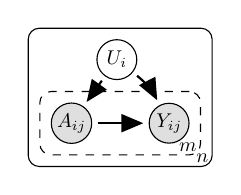
\begin{tikzpicture}[scale=0.72, transform shape]
\node[obs] (y) {$Y_{ij}$};
\node[obs, left=1cm of y] (a) {$A_{ij}$};
\node[latent, above=0.4cm of a, xshift=0.8cm] (u) {$U_i$};
\draw[hcmarrow] (a) -- (y);
\draw[hcmarrow] (u) to[bend left=12] (y);
\draw[hcmarrow] (u) -- (a);
\plate[dashed] {in} {(a)(y)} {$m$}
\plate {out} {(in)(u)} {$n$}
\end{tikzpicture}
\end{minipage}\hspace{0.01\textwidth}
\begin{minipage}[t]{0.23\textwidth}
\centering
\textbf{(b) Collapsed}\par\medskip
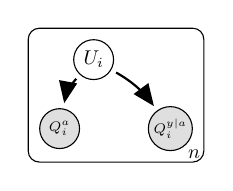
\begin{tikzpicture}[scale=0.72, transform shape]
\node[obs] (qya) {$\scriptstyle Q^{y \mid a}_i$};
\node[obs, left=1.2cm of qya] (qa) {$\scriptstyle Q^{a}_i$};
\node[latent, above=0.5cm of qa, xshift=0.6cm] (u) {$U_i$};
\draw[hcmarrow] (u) to[bend right=16] (qa);
\draw[hcmarrow] (u) to[bend left=12] (qya);
\plate {ayu} {(qa)(qya)(u)} {$n$}
\end{tikzpicture}
\end{minipage}\hspace{0.01\textwidth}
\begin{minipage}[t]{0.23\textwidth}
\centering
\textbf{(c) Augmented}\par\medskip
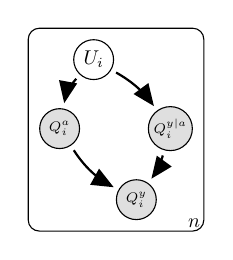
\begin{tikzpicture}[scale=0.72, transform shape]
\node[obs] (qya) {$\scriptstyle Q^{y \mid a}_i$};
\node[obs, left=1.2cm of qya] (qa) {$\scriptstyle Q^{a}_i$};
\node[latent, above=0.5cm of qa, xshift=0.6cm] (u) {$U_i$};
\node[obs, below=0.5cm of qya, xshift=-0.6cm] (qy) {$\scriptstyle Q^{y}_i$};
\draw[hcmarrow] (u) to[bend right=16] (qa);
\draw[hcmarrow] (u) to[bend left=12] (qya);
\draw[hcmarrow] (qa) to[bend right=14] (qy);
\draw[hcmarrow] (qya) to[bend left=10] (qy);
\plate {ayu} {(qa)(qya)(qy)(u)} {$n$}
\end{tikzpicture}
\end{minipage}\hspace{0.01\textwidth}
\begin{minipage}[t]{0.23\textwidth}
\centering
\textbf{(d) Marginalized}\par\medskip
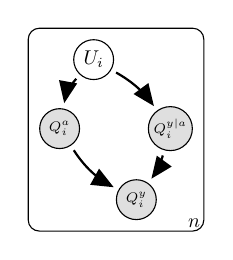
\begin{tikzpicture}[scale=0.72, transform shape]
\node[obs] (qya) {$\scriptstyle Q^{y \mid a}_i$};
\node[obs, left=1.2cm of qya] (qa) {$\scriptstyle Q^{a}_i$};
\node[latent, above=0.5cm of qa, xshift=0.6cm] (u) {$U_i$};
\node[obs, below=0.5cm of qya, xshift=-0.6cm] (qy) {$\scriptstyle Q^{y}_i$};
\draw[hcmarrow] (u) to[bend right=16] (qa);
\draw[hcmarrow] (u) to[bend left=12] (qya);
\draw[hcmarrow] (qa) to[bend right=14] (qy);
\draw[hcmarrow] (qya) to[bend left=10] (qy);
\plate {ayu} {(qa)(qya)(qy)(u)} {$n$}
\end{tikzpicture}
\end{minipage}
\caption{Complete graph transformations for the confounder motif. The collapsed graph exposes $Q^a_i$ and $Q^{y\mid a}_i$ as unit-level random variables confounded by $U_i$; augmentation adds the target $Q^y_i$.}
\label{fig:complete-confounder}
\end{figure}


\begin{figure}[!htbp]
\centering
\normalsize
\begin{minipage}[t]{0.31\textwidth}
\centering
\textbf{(a) HCM}\par\medskip
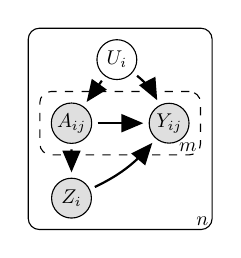
\begin{tikzpicture}[scale=0.72, transform shape]
\node[obs] (y) {$Y_{ij}$};
\node[obs, left=1cm of y] (a) {$A_{ij}$};
\node[latent, above=0.4cm of a, xshift=0.8cm] (u) {$U_i$};
\node[obs, below=.6cm of a] (z) {$Z_i$};
\draw[hcmarrow] (a) -- (y);
\draw[hcmarrow] (u) to[bend left=12] (y);
\draw[hcmarrow] (u) -- (a);
\draw[hcmarrow] (a) -- (z);
\draw[hcmarrow] (z) to[bend right=12] (y);
\plate[dashed] {in} {(a)(y)} {$m$}
\plate {out} {(in)(u)(z)} {$n$}
\end{tikzpicture}
\end{minipage}\hspace{0.015\textwidth}
\begin{minipage}[t]{0.31\textwidth}
\centering
\textbf{(b) Collapsed}\par\medskip
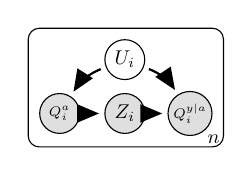
\begin{tikzpicture}[scale=0.72, transform shape]
\node[obs] (qa) at (-1.15,0) {$\scriptstyle Q^{a}_i$};
\node[obs] (z) at (0,0) {$Z_i$};
\node[obs] (qya) at (1.15,0) {$\scriptstyle Q^{y \mid a}_i$};
\node[latent] (u) at (0,0.95) {$U_i$};
\draw[hcmarrow] (u) to[bend right=18] (qa);
\draw[hcmarrow] (u) to[bend left=18] (qya);
\draw[hcmarrow] (qa) -- (z);
\draw[hcmarrow] (z) -- (qya);
\plate {ayu} {(qa)(qya)(u)(z)} {$n$}
\end{tikzpicture}
\end{minipage}\hspace{0.015\textwidth}
\begin{minipage}[t]{0.31\textwidth}
\centering
\textbf{(c) Augmented}\par\medskip
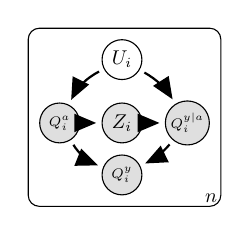
\begin{tikzpicture}[scale=0.72, transform shape]
\node[obs] (qya) {$\scriptstyle Q^{y \mid a}_i$};
\node[obs, left=1.5cm of qya] (qa) {$\scriptstyle Q^{a}_i$};
\node[obs, left=.4cm of qya] (z) {$Z_i$};
\node[latent, above=.4cm of z] (u) {$U_i$};
\node[obs, below=.2cm of z] (qy) {$\scriptstyle Q^{y}_i$};
\draw[hcmarrow] (u) to[bend right=18] (qa);
\draw[hcmarrow] (u) to[bend left=14] (qya);
\draw[hcmarrow] (qa) -- (z);
\draw[hcmarrow] (z) -- (qya);
\draw[hcmarrow] (qa) to[bend right=18] (qy);
\draw[hcmarrow] (qya) to[bend left=12] (qy);
\plate {ayu} {(qa)(qy)(qya)(u)(z)} {$n$}
\end{tikzpicture}
\end{minipage}
\caption{Complete graph transformations for the confounder-and-interference motif. The collapsed graph has a frontdoor-like path $Q^a_i \to Z_i \to Q^{y\mid a}_i$, and augmentation adds the target $Q^y_i$.}
\label{fig:complete-interference}
\end{figure}

\section{Effective graph diagnostic}
\label{app:effective-graph}
The effective graph in Figure~\ref{fig:exactbic-effective-graph} is reported in the appendix because it documents the stabilized ExactBIC computation rather than the main STAR estimand itself.

\begin{figure}[!htbp]
\centering
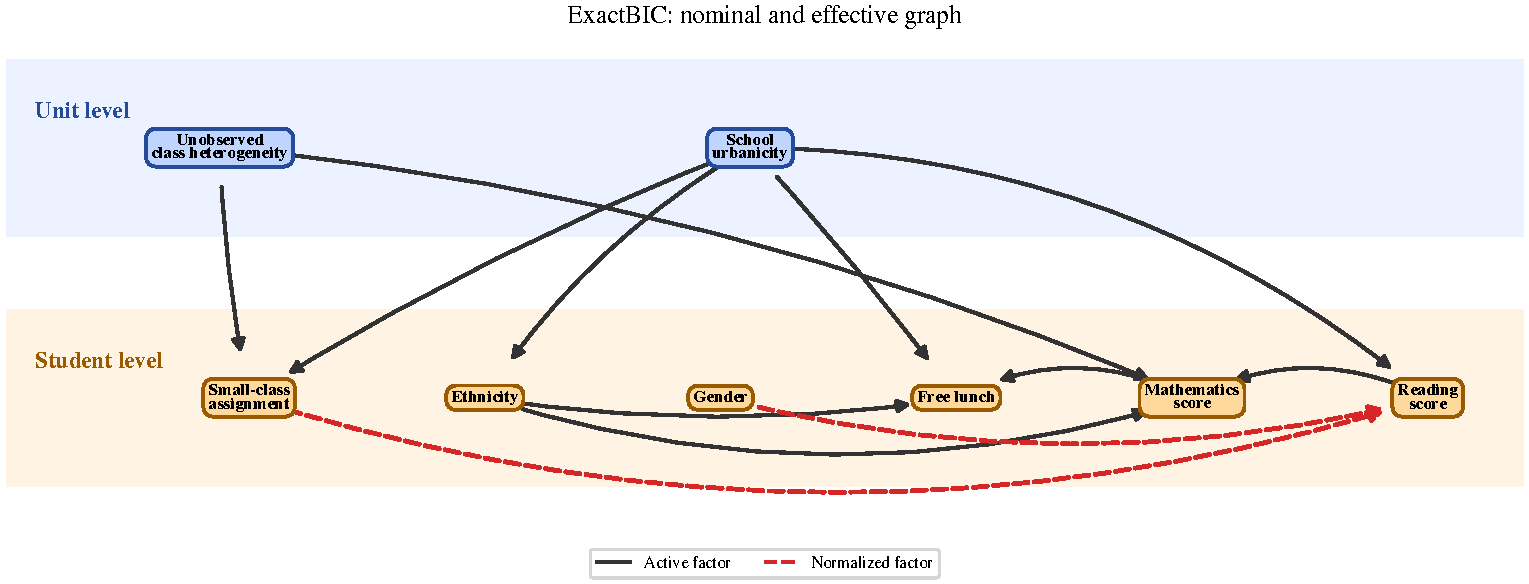
\includegraphics[width=0.96\textwidth]{ExactBIC_with_factor1_effective_graph_curved.pdf}
\caption{ExactBIC-derived HCM graph with normalized factors. Dashed red arrows mark dependencies whose multiplicative factors are normalized for numerical stability in the stabilized evaluation.}
\label{fig:exactbic-effective-graph}
\end{figure}

\section{Additional STAR tail diagnostics}
\label{app:tail-diagnostics}
Figure~\ref{fig:score-hist-diagnostics} provides the histogram counterpart to the Q-Q tail diagnostic reported in the main text.
It is included as a modelling check for the Gaussian plug-in approximation, not as a separate substantive result.

\begin{figure}[!htbp]
\centering
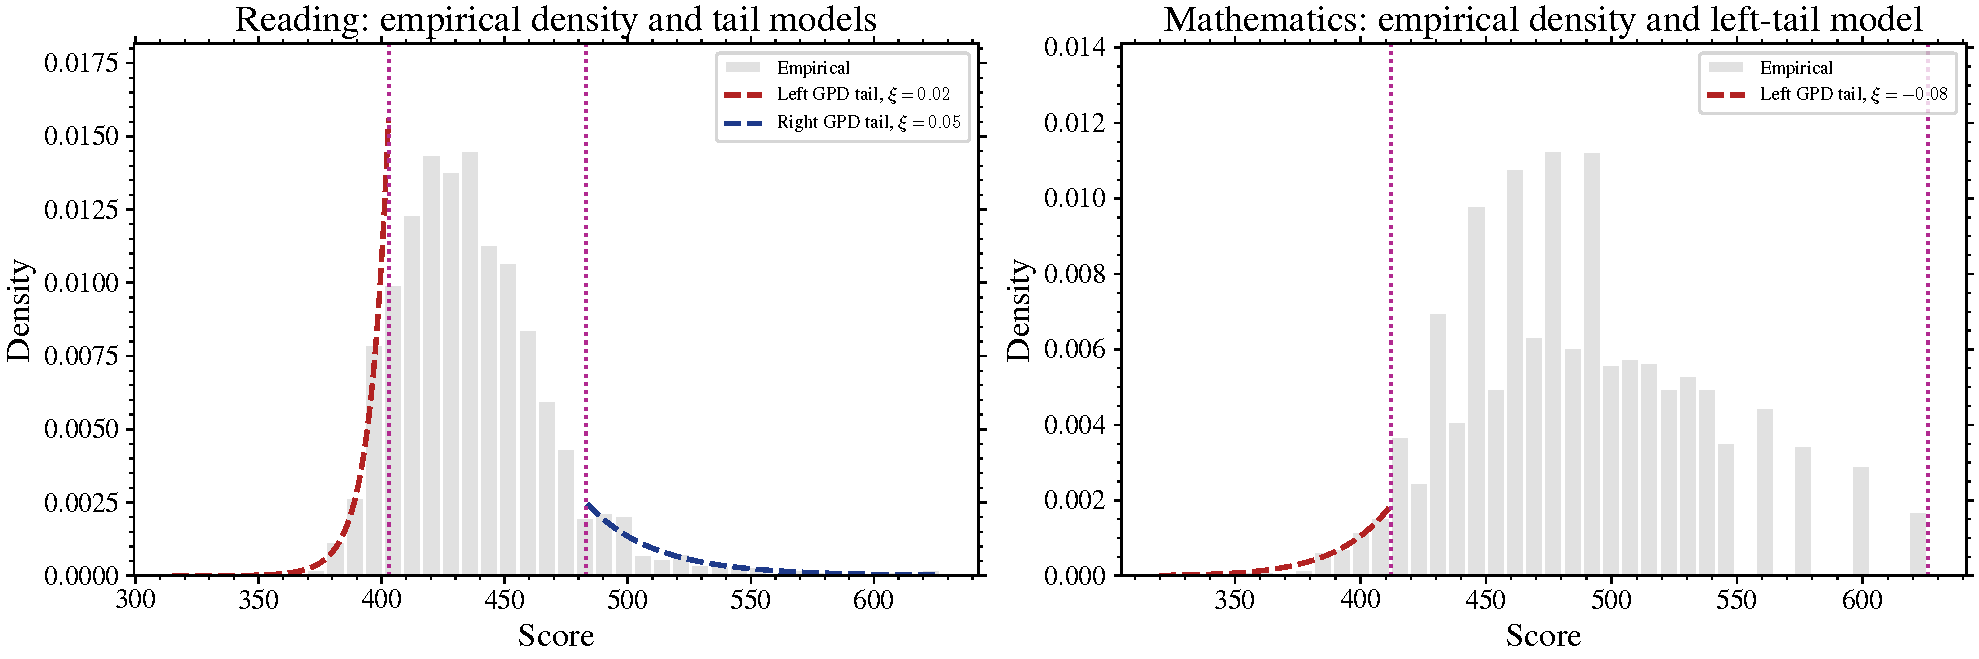
\includegraphics[width=0.86\textwidth]{global_Y_M_heavy_tail_hist.pdf}
\caption{Heavy-tail histogram diagnostics for Reading ($Y$) and Mathematics ($M$). Empirical score densities are shown with GPD-type tail fits, confirming that the STAR score distributions have heavy non-Gaussian tails.}
\label{fig:score-hist-diagnostics}
\end{figure}

\section{Additional synthetic benchmarks}
\label{app:synthetic-benchmarks}
The additional benchmark scenarios in Table~\ref{tab:benchmarks} are included as implementation checks.
They are not intended to define new estimands for the STAR analysis; their role is to verify that the code behaves as expected in controlled settings where the target is known.

\begin{table}[!htbp]
\centering
\caption{Representative benchmark scenarios used as synthetic implementation checks.}
\label{tab:benchmarks}
\begin{tabular}{lccc}
\toprule
Scenario & Ground truth & HCM/per-unit & Naive OLS \\
\midrule
Binary confounder & 0.315 & 0.363 & -- \\
Spatio-temporal confounder & 5.00 & 5.10 & 27.1 \\
Spatio-temporal dynamics & 5.00 & 5.10 & 33.0 \\
Grouped socioeconomic outcome & 0.35 log & 0.34 & 0.70 \\
\bottomrule
\end{tabular}
\end{table}

\section{Software notes}
\label{app:software-notes}
The implementation provides graph transformations, do-calculus identification, AST evaluation, parametric and neural estimators, and STAR replication scripts. The current draft reports the stable artefacts used for the STAR analysis. The code is available at \href{https://github.com/AI-vidence/hierarchicalcausalmodels}{this link}.

\begin{table}[!htbp]
\centering
\small
\caption{Parallel estimation structure for the three canonical HCM motifs. The CPU column reports the work after splitting independent tasks across $P=4$ workers. The GPU implementation uses the same independent tasks, but batches them as tensors; the feasible batch size is measured separately as a function of $(n,m)$ rather than treated as a fixed worker count.}
\label{tab:motifs}
\begin{tabular}{lccc}
\toprule
Motif & Independent tasks & Sequential work & CPU work, $P=4$ \\
\midrule
Confounder & $n$ response tasks & $nc$ & $\lceil n/4\rceil c$ \\
Confounder and interference & $2n$ response/mediator tasks & $2nc$ & $\lceil 2n/4\rceil c$ \\
Instrument & $3n$ instrument/weight tasks & $3nc$ & $\lceil 3n/4\rceil c$ \\
\bottomrule
\end{tabular}
\end{table}

The GPU benchmark in Figure~\ref{fig:gpu-pareto-frontier} should be read as a regime diagnostic.
On the local consumer GPU, small and moderate workloads are often dominated by data movement and CUDA launch overhead, so speedups become meaningful only when $n\times m$ is large enough to keep the device saturated.
The same script is therefore intended to be rerun on accelerator hardware with larger memory and bandwidth, such as an H100, before drawing conclusions about production-scale GPU speedups.

\begin{figure}[!htbp]
\centering
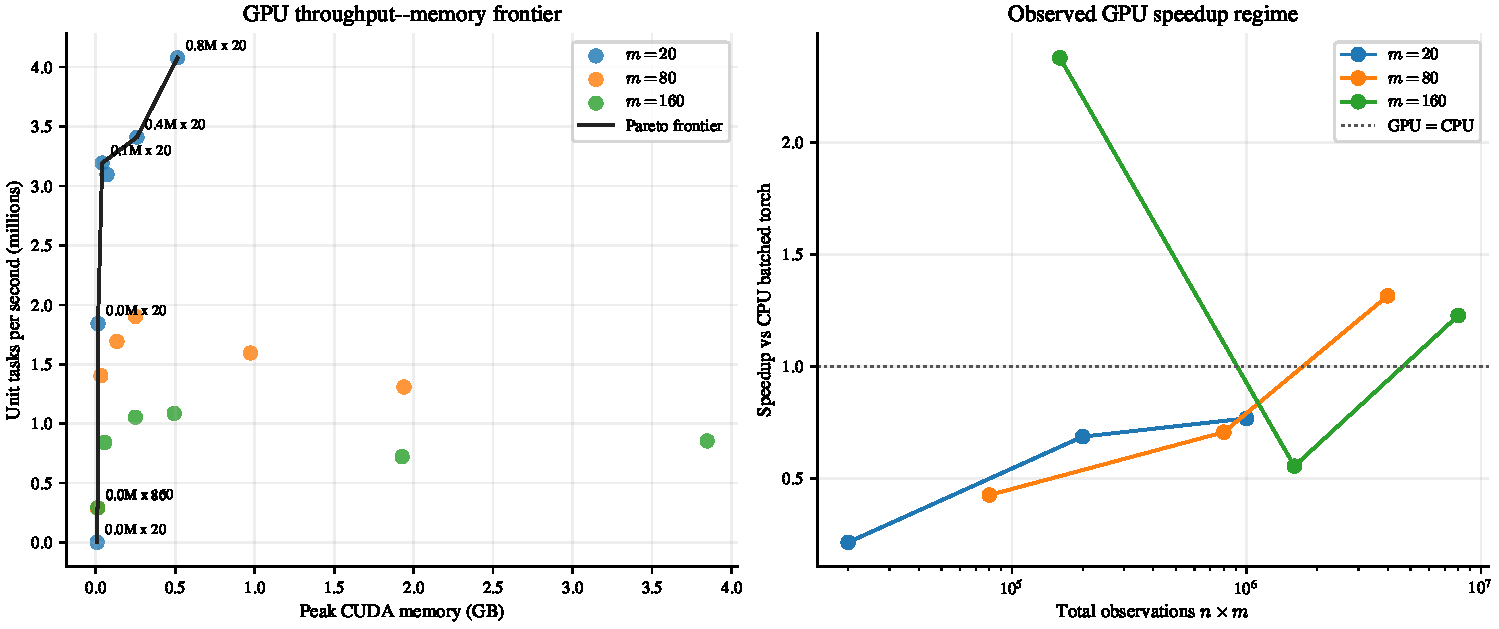
\includegraphics[width=0.88\textwidth]{gpu_hcm_pareto_frontier.pdf}
\caption{Hardware-specific Pareto benchmark for batched GPU HCM evaluation. Each point corresponds to one synthetic batched Gaussian HCM workload with a given number of units $n$ and sub-units $m$. The left panel reports the throughput--memory trade-off and highlights non-dominated CUDA points; the right panel reports the observed speedup over the batched CPU torch baseline for workloads where the CPU baseline was also measured, with the dotted line marking parity. On the local RTX 4060 Laptop GPU, the main message is the onset of a GPU-beneficial regime rather than uniformly large speedups; larger accelerators should move this frontier upward and outward.}
\label{fig:gpu-pareto-frontier}
\end{figure}
\end{appendices}

\end{document}
